%\part{title}% Source: http://tex.stackexchange.com/a/5374/23931
\documentclass[12pt]{article}
%\usepackage[turkish,english]{babel}
%\usepackage[T1]{fontenc}
\usepackage[utf8]{inputenc}
\usepackage[margin=1in]{geometry}
\usepackage[11pt]{moresize}
\usepackage{}

\usepackage{textcomp}

\usepackage[pdftex, bookmarksopen=true]{hyperref}
\usepackage[all]{hypcap}

\usepackage{amsmath}
\usepackage{mathtools}
\usepackage{listings}
\usepackage{tocbibind}
\usepackage{hyperref}
\usepackage{color}
\usepackage{textcomp}
\usepackage{geometry}
\usepackage{xcolor}
\usepackage{amsmath}
\usepackage[most]{tcolorbox}
\usepackage{amssymb}
\usepackage{pifont}
\usepackage{ulem}
\usepackage{cancel}
\usepackage{tikz}
\usepackage{fourier-orns}
\usepackage{longtable}
\usepackage{bm}
\usepackage{siunitx}
\usepackage{graphicx}

\usepackage{bookmark}

\usepackage{upgreek}
\usepackage[toc,page]{appendix}

\usepackage{mathtools}    % loads »amsmath«


\definecolor{mygreen}{RGB}{28,172,0} % color values Red, Green, Blue
\definecolor{mylilas}{RGB}{170,55,241}

\allowdisplaybreaks


\newcommand{\HRule}{\rule{\linewidth}{0.5mm}}
\newcommand{\Hrule}{\rule{\linewidth}{0.3mm}}

\DeclareMathOperator{\atantwo}{atan2}

\DeclarePairedDelimiter{\norm}{\lVert}{\rVert} 

\usepackage{xcolor}
\usepackage[linesnumbered,ruled,vlined]{algorithm2e}
\usepackage{algorithmic}
%%% Coloring the comment as blue
% comment style (algorithms)
\newcommand{\xCommentSty}[1]{\scriptsize\ttfamily\textcolor{blue}{#1}}
\SetCommentSty{xCommentSty}
%%%
\SetKwInput{KwInput}{Input}                % Set the Input
\SetKwInput{KwOutput}{Output}              % Set the Output
\SetKwInput{KwInitalize}{Initialize}       % set the Initialize

\DeclarePairedDelimiter\ceil{\lceil}{\rceil}
\DeclarePairedDelimiter\floor{\lfloor}{\rfloor}
\newcommand{\Mod}[1]{\ (\mathrm{mod}\ #1)}

\usepackage{subfig}

\newcommand{\nosemic}{\renewcommand{\@endalgocfline}{\relax}}% Drop semi-colon ;
\newcommand{\dosemic}{\renewcommand{\@endalgocfline}{\algocf@endline}}% Reinstate semi-colon ;
\newcommand{\pushline}{\Indp}% Indent
\newcommand{\popline}{\Indm\dosemic}% Undent
\let\oldnl\nl% Store \nl in \oldnl
\newcommand{\nonl}{\renewcommand{\nl}{\let\nl\oldnl}}% Remove line number for one line

\makeatletter% since there's an at-sign (@) in the command name
\renewcommand{\@maketitle}{%
	\parindent=0pt% don't indent paragraphs in the title block
	\centering
	{\Large \bfseries\textsc{\@title}}
	\HRule\par%
	\textit{\@author \hfill \@date}
	\par
}
\makeatother% resets the meaning of the at-sign (@)

\title{Report: Parameter Identification and State Estimation of an Battery by Using Second Order Equivalent Circuit Model}
\author{İ. Ç. Yılmaz}
\date{Apr 23, 2021}

\renewcommand\refname{References}

\lstset{language=Matlab,%
	%basicstyle=\color{red},
	breaklines=true,%
	morekeywords={matlab2tikz},
	keywordstyle=\color{blue},%
	morekeywords=[2]{1}, keywordstyle=[2]{\color{black}},
	identifierstyle=\color{black},%
	stringstyle=\color{mylilas},
	commentstyle=\color{mygreen},%
	showstringspaces=false,%without this there will be a symbol in the places where there is a space
	numbers=left,%
	numberstyle={\tiny \color{black}},% size of the numbers
	numbersep=9pt, % this defines how far the numbers are from the text
	emph=[1]{for,end,break},emphstyle=[1]\color{red}, %some words to emphasise
	%emph=[2]{word1,word2}, emphstyle=[2]{style},  
}

\makeatletter
\setlength{\@fptop}{0pt}
\makeatother

\begin{document}
\maketitle% prints the title block

\section{Introduction} \label{Introduction}
\par It is well known that accurate identification of the key state parameters and State of Charge (SOC) estimation method for a Li-ion battery cell is of great significance for advanced battery management system (BMS) of electric vehicles (EVs). Systematic experimental data-driven parameter identification techniques and sophisticated SOC estimation algorithms (also can be called as filtering algorithm) for a battery equivalent circuit model in EV applications. The key state parameters of the battery cell were identified based on the second-order resistor capacitor (RC) equivalent circuit model \cite{Pang2018}. \newline

\par \noindent For EVs and HEVs, the accurate state parameters and state-of-charge (SOC) of an battery is of great significance in \underline{real-time control} and \underline{high-performance operation} for advanced battery management system (BMS) of EVs because these parameters are often used to implement the optimum control of charging and discharging process, which is not only beneficial for efficient vehicular BMS, but also for the diagnosis and prognosis of the battery behavior. Therefore, it is necessary to obtain the inner state
parameters and to make an accurate SOC estimation for the battery accurately \cite{Pang2018}.\newline

\begin{figure}[t!]
	\centering
	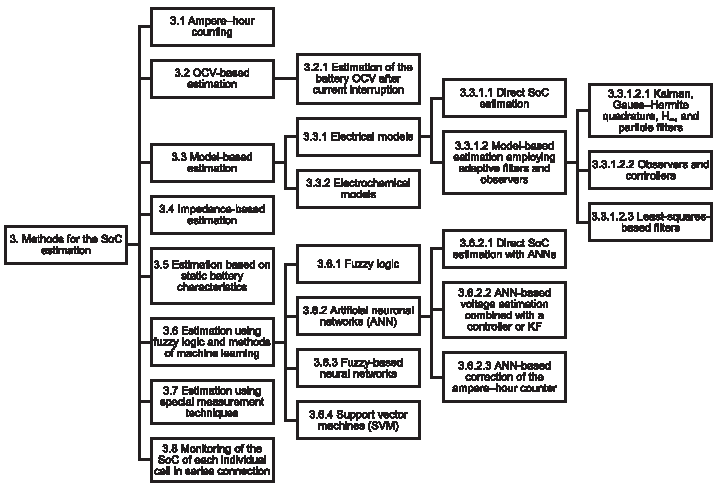
\includegraphics[width=0.80\textwidth, keepaspectratio]{images/Classification_of_the_methods_for_the_SoC_estimation.pdf}
	\caption{Classification of the methods for the SOC estimation. \cite{WaaG2014}}
	\label{fig:Classification_of_the_methods_for_the_SOC_estimation}
\end{figure}

\par \noindent There are a wide range of
approaches proposed in the 
literature, most of which can be seen in the Fig \ref{fig:Classification_of_the_methods_for_the_SOC_estimation}. In this study, model-based estimation strategy with electrical models are intended to identify key parameters of the second order equivalent circuit. Adaptive filters and some observers are extensively employed for estimating the SOC. These filter and observer may include separate or collaborative usage of the Kalman Filter (KF), Extended Kalman Filter (EKF), Unscented Kalman Filter (UKF), particle filters, and Least-squares-based filters  due to batteries' closed-loop nature
and concerning various uncertainties. \newline 

\par \noindent As the battery capacity, the impedance parameters of the battery (RC parameters) in a new state are mainly defined by the battery design, but changes significantly over the lifetime due to aging processes. The knowledge of the present battery impedance parameters is mainly required for

\begin{figure}[t!]
	\centering
	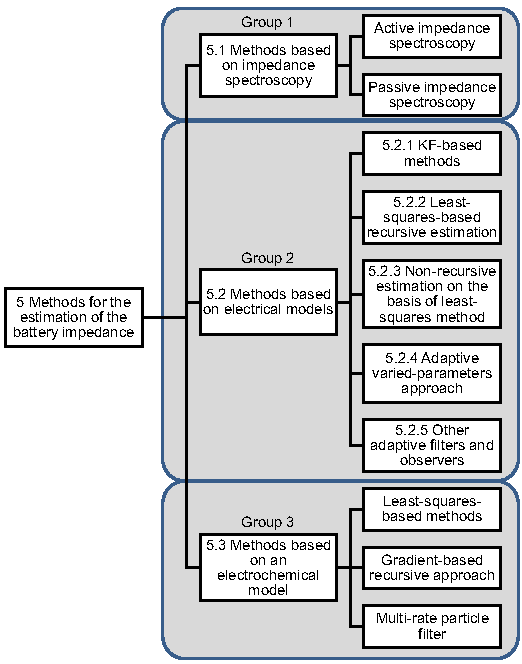
\includegraphics[width=0.70\textwidth, keepaspectratio]{images/Classification_of_the_methods_for_the_estimation_of_the_battery_impedance.pdf}
	\caption{Classification of the methods for the estimation of the battery impedance.\cite{WaaG2014}}
	\label{fig:Classification_of_the_methods_for_the_estimation_of_the_battery_impedance}
\end{figure}

\begin{itemize}
	\item estimation of the energy losses in the battery during the
operation,
	\item SOC estimation based on electrical models,
	\item prediction of the available power of the battery.
\end{itemize}

\par \noindent Especially for the latest task the impedance parameters must be determined very accurate including their dependence on the current. All methods for the estimation of the battery impedance can be divided into the three groups and the mentioned groups can be seen in Fig \ref{fig:Classification_of_the_methods_for_the_estimation_of_the_battery_impedance}.

\section{An Equivalent Second-Order Circuit Model (ECM) of An Battery} \label{Model}
The research showed that the second-order RC model has the highest precision and is more suitable for the voltage estimation of battery cells. He et. al. \cite{He2012} use online parameter identification method to determine the relationship between the model accuracy and the number of RC networks, and concluded that the model with a second-order RC network has the best performance. \newline

\par \noindent As shown in Fig \ref{fig:Schematic_diagram_of_the_second_order_RC_model}, the second-order
RC battery model is composed of an open-circuit voltage (OCV) denoted by $U_{oc}(SOC)$ which is a function of SOC, a resistance $R_{\Omega}$,
 and two parallel RC networks connected in series (i.e., $R_{1}=R_{ep}$, $C_{1}=C_{ep}$ and $R_{1}=R_{cp}$ ,$C_{1}=C_{cp}$). The resistance $R_{\Omega}$ is the Ohmic resistances caused by the accumulation and dissipation of charge in the electrical double-layer; $R_{1}$
and $C_{1}$ are the electro-chemical polarization resistance and capacitance, respectively; $R_{2}$ and $C_{2}$ are
the concentration polarization resistance and capacitance, respectively; $U_{1}=U_{ep}$ and $U_{cp}$ are the polarization
 voltage across $C_{1}$ and $C_{2}$, respectively; $I(t)$ is the load current (supposed positive for discharge and
negative for charge); and $U_{t}$ is battery the terminal voltage. \newline

\begin{figure}[b!]
	\centering
	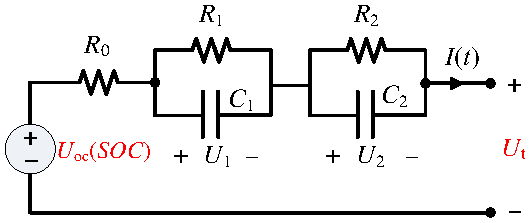
\includegraphics[height=0.20\textwidth, keepaspectratio]{images/Schematic_diagram_of_the_second_order_RC_model.pdf}
	\caption{Schematic diagram of the second-order RC model.}
	\label{fig:Schematic_diagram_of_the_second_order_RC_model}
\end{figure}

\par \noindent The electrical behavior of the second-order RC battery model can
be governed in the continuous time domain by following three equations as follows:

\begin{subequations} 
	\label{eqn:electrical_behavior_of_the_proposed_model}
	\begin{align} \dot{U}_{1}(t) &= -\frac{1}{R_{1}C_{1}}U_1(t) + \frac{1}{C_1}I(t) \\ 
	\dot{U}_{2}(t) &= -\frac{1}{R_{2}C_{2}}U_2(t) + \frac{1}{C_2}I(t) \\ 
		U_{t}(t) &= U_{oc}(SOC)(t) - {U}_{1}(t) - {U}_{2}(t) - I(t)R_{0} 
	\end{align} 
\end{subequations}

\par \noindent Mathematical relations involving SOC in continuous time domain can be written as follows:

\begin{equation}
	\label{eqn:SOC_in_continious_time}
	SOC(t) = SOC(t_{0}) - \frac{1}{Q}\int_{t_{0}}^{t}\eta I(\uptau)d\uptau
\end{equation}

\noindent or 

\begin{equation}
	\label{eqn:SOC_in_continious_time_without_integral}
	\dot{SOC(t)} = -\frac{\eta I(t)}{Q}
\end{equation}

\noindent where $I(t)$ is instantaneous cell current (assumed positive for discharge, negative for charge). The sign of $I(t)$ is positive on discharge. Hence, positive (discharge) current lowers the cell’s state of charge, and negative (charge) current increases the cell’s state of charge. Care must be taken with units: $I(t)$ is measured in amperes, and to be compatible, Q must be converted to ampere-seconds (i.e., coulombs) \cite{Plett2015}. $Q$ is the cell nominal capacity. Cell Coulombic efficiency $\eta$ is $\eta=1$ for discharge, and $\eta = \eta \leq 1 $  for charge. Using a rectangular approximation for integration and a "suitably small" sampling period $\Delta{t}$, a discrete-time approximate recurrence may then be written as

\begin{equation}
	\label{eqn:SOC_in_discrete_time}
	SOC[k+1] = SOC[k] - \bigg(\frac{\eta\Delta{t}}{Q}\bigg)I[k] \
\end{equation}

\noindent where $SOC[k + 1]$ and $SOC[k]$ are the $SOC$ at $
[k + 1]$th and $k$th sampling time, respectively; $\eta$ is
the Coulomb efficiency that is assumed to be 1 at charging and 0.98 at discharging as the battery works in a limited current range. Then, the continuous time state-space representation with \ref{eqn:electrical_behavior_of_the_proposed_model}, \ref{eqn:SOC_in_continious_time_without_integral} can be written as:

\begin{equation}
	\label{eqn:continues_time_state_space}
	Continuous~Time~LTI~State~Space
	\begin{cases}
		& \dot{\bm{x}}(t) = \bm{A}\bm{x}(t)\,+\,\bm{B}u(t)  \\
		& h(t) = {y}(t) - U_{OC}(SOC(t)) = \bm{C}\bm{x}(t)\,+\,{D}u \\
	\end{cases}   
\end{equation} 

\noindent where $\bm{A} = \begin{bmatrix} -\frac{1}{R_{1}C_{1}} & 0 & 0  \\ 0 & -\frac{1}{R_{2}C_{2}} & 0 \\ 0 & 0 & 0 \end{bmatrix}$, $\bm{B} = \begin{bmatrix} \frac{1}{C_{1}} \\ \frac{1}{C_{2}} \\ -\frac{\eta}{Q}  \end{bmatrix}$,  $\bm{C} = \begin{bmatrix} -1 & -1 & 0 \end{bmatrix}$, $D = R_{0}$. State vector of the state space system is denoted by $\bm{x} = [U_{1}\,\,U_{2}\,\,SOC]^T$ and $u(t) = I(t)$ indicates the input of the battery system and $y(t) = U_t(t)-U_{OC}(SOC)$ is the output. %$\bm{w}$ and $v$ are the observation noise and measurement noise respectively.

\section{SOC - OCP Relationship} \label{SOC_OCP_Relationship}

The SOC-OCV function is therefore representative for a particular battery, and is generally a nonlinear monotone function between SOC and OCV for all lithium-ion batteries. It is hence widely used in battery management systems (BMS) for correcting SOC calculation.\cite{Zhang2016} The accuracy of the SOC-OCV curve has great influence on the SOC value estimated.It is consequently important to determine the SOC-OCV relationship precisely, if an accurate estimation of the battery state is necessary. \newline

\begin{figure}[t!]
	\centering
	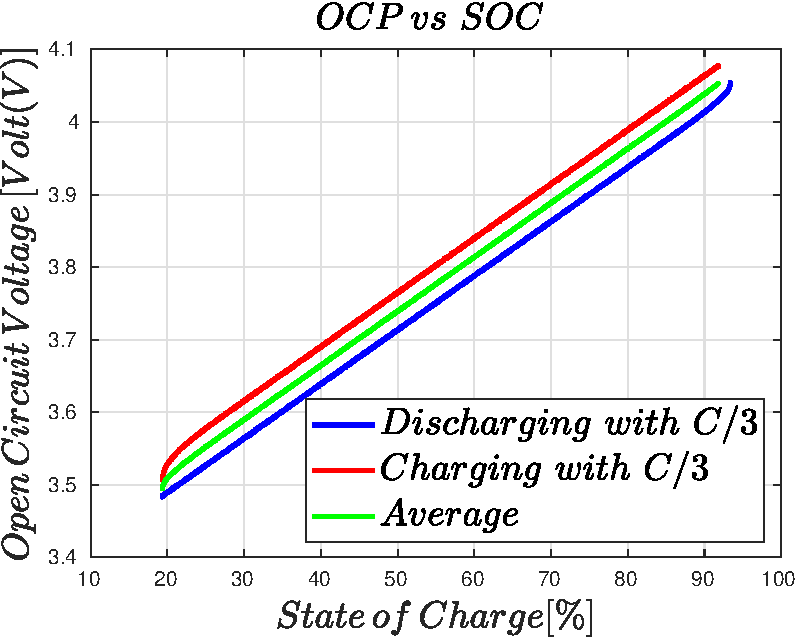
\includegraphics[width=0.6\textwidth, keepaspectratio]{images/OCV_vs_SOC.pdf}
	\caption{Experimental SOC-OCV mapping when battery is charged/discharged with $C/3$ capacity.}
	\label{fig:OCV_vs_SOC}
\end{figure}

\par \noindent \textbf{NOTE [Verification of OCV Model]}: To validate the proposed OCV model, a series of experiments are performed on different classes of batteries to obtain SOC-OCV mapping data. Some experiment is performed with the battery charged from its fully discharged state at a current of 0.05 C. The charging continued until the terminal voltage of the battery reached the charging voltage limit. The battery was subsequently open-circuited for 2 h, after being discharged at 0.05 C until the battery terminal voltage reached the discharge voltage limit.
Taking the average potential between the charge and discharge branch at $C/20$ or $C/30$  and the normalized $C/20$ or $C/30$ capacity, the voltage and its corresponding SOC can be regarded as OCV versus SOC curve \cite{Dubarry2007}\newline 

\par \noindent To reach a acceptable OCV-SOC relation, three OCV models are selected in the literature and all of them is compared to each others. All of the parameters in the OCV models are indicated \ref{table:Comparing_Fitting_Results} and they are found by employing the MATLAB \href{https://www.mathworks.com/products/curvefitting.html}{\textit{Curve Fitting}} toolbox in R2018b. All three screenshot of the curve fittings and related plots can be found at the Appendix \ref{Curve_Fitting_Appendeix} section.

\subsection{Matlab Code to Obtain OCV-SOC RelationShip}
In this code snippet, 'SoC\_OCV\_x\_axis' and 'SoC\_OCV\_Y\_axis' vectors are employed in the curve fitting. The SOC of the battery is taken between 0 and 1 instead of percentage value.  
\lstinputlisting{MATLAB_Files/OCV_SOC_Data.m} 

\begin{table}[!b]
	\begin{tabular}{c | c | c | c } 
		\hline
		\# & OCV Model & Reference & RMS Error (mV)\\ [0.5ex] 
		\hline\hline
		$1$ & $U_{OC}(s) = a  + b \times (-ln(s))^m + c \times s + d \times \exp^{n(s-1)}$ & \cite{Zhang2016} & $0.4798$ \\ 
		\hline
		$2$ & $U_{OC}(s) = K_{0} - \frac{K_{1}}{s} - K_{2}s + K_{3}ln(s) + K_{4}ln(1 - s)$  & \cite{Plett2004} & $0.2431$ \\ 
		\hline
		$3$ & $U_{OC}(s) = K_{0} + K_{1}{\exp}^{-\alpha(1-s)} - \frac{K_{2}}{s}$  & \cite{Neumann2011} & $0.3060$ \\ 
		\hline
	\end{tabular}
	\caption{\label{table:Comparing_Fitting_Results}Compared fitting results of OCV models.}
\end{table}

\par \noindent The RMSE value of each model is taken as a criterion for selection of the most suitable OCV model. It can be understood that more precise experiment must be done to be reached the appropriate OCV-SOC models. In literature, batteries is charged and discharged nearly at $C/20$ or $C/30$. Then the average potential between the charge and discharge branch is calculated to achieve experimental OCV-SOC curvature. The purpose of the slow rate is to minimize the excitation of the
dynamic parts of the cell model. The cell in a quasi-equilibrium state is desired to keep  at all times. So, $C/30-C/20$ rate is generally used for which is a compromise between the desire to have zero current to have a
true equilibrium and the practical realization that the test will already require on the order of 40 to 60 h to complete within above mentioned charge and discharged levels. Model - 2 is employed to able to associate between OCV and SOC in this study with the parameters found in \ref{Model-2} \textbf{In the given data, slow charging and and discharging was not performed during the experiment, so that charging and discharging with $C/3$ capacity rate is taken into consideration}.

\section{Parameters Identification of the Battery Model} 
\label{Parameter_Identification_Section}

\subsection{Preliminary Work}
\label{Parameter_Identification_Preliminary_Work}

To identify the model parameters, a constant-current discharge pulse
is  generally subjected to the cell and then the cell is allowed
to rest while recording the cell’s voltage response during a fair amount of time \cite{Plett2015}. A model type of sort having a single parallel resistor–capacitor subcircuit is assumed to this point, exactly as drawn in Fig \ref{fig:Response_to_discharge_pulse}. \newline 

\begin{figure}[t!]
	\centering
	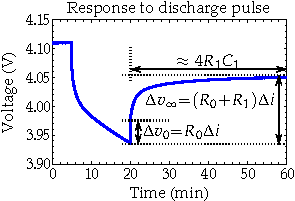
\includegraphics[width=0.5\textwidth, keepaspectratio]{images/Parameter_values_from_a_pulse_response.pdf}
	\caption{ Measuring parameter values
from a pulse response for first order circuit \cite{Plett2015}.}
	\label{fig:Response_to_discharge_pulse}
\end{figure}

\par \noindent Total capacity denoted by the symbol Q is a parameter of the cell model; that is, it is
a constant that may differ from cell to cell. Total capacity is not a
function of temperature or current. It is not taken into consideration in the parameter identification calculation, its value is directly obtained from the first discharge step which is given in the experimental data by using discrete time equation \ref{eqn:SOC_in_discrete_time}. The MATLAB code in Appendix \ref{Total_Capacity_Calculation} snippet is used in the calculation of Q value. Note that the coulombic efficiency, $\eta(t)$ is adopted $1$ for discharging. \newline      

\par \noindent The circuit of the battery battery model however includes extra concentration polarization resistance and capacitance, $R_{2}$ and $C_{2}$, respectively. Instead of making an rough mathematical calculation that is explained in detail literature, constrained optimization problem is solved to find parameter values in the time interval between constant current discharge pulse and rest time. Model parameters includes $R_{0}$, $R_{1}$, $\tau_{1}$, $R_{2}$ and $\tau_{2}$. Sometimes ohmic resistance value, $R_{0}$, is separately calculated for charging, $R_{0}^{-}$, and discharging, $R_{0}^{+}$, process. For the sake of simplicity, $R_{0}$ is only identified from discharging pulse. Time constants, $\tau_{1}=R_{1}C_{1}$ and $\tau_{2}=R_{2}C_{2}$ are sometimes utilized as parameters rather than using resistor values $C_{1}$ and $C_{2}$. Eventually, parameter vector can be written as $\bm{\Theta} = [R_{0}\,\,R_{1}\,\,\tau_{1}\,\,R_{2}\,\,\tau_{2}]^{T}$. By using experimental data, the constant current discharge pulse start at $t=28785$ sec and continues until $t=31109$ sec. Then, battery is allowed to rest approximately half an hour (Rest time finishes at $t = 31109$ sec). The Fig includes the current and terminal voltage measurements during the above mentioned intervals. As it can be understood that, voltage characteristic of the battery at this region resembles like the behaviour which is already mentioned at the beginning of this chapter. State of charge (SOC) is also saved in this interval to calculate OCV of the battery. Total capacity of the battery is found as $Q=1129.4$ Ampere-second or $313.7$ milli-Ampere hour (mAh). \newline

\begin{figure}[t!]
	\centering
	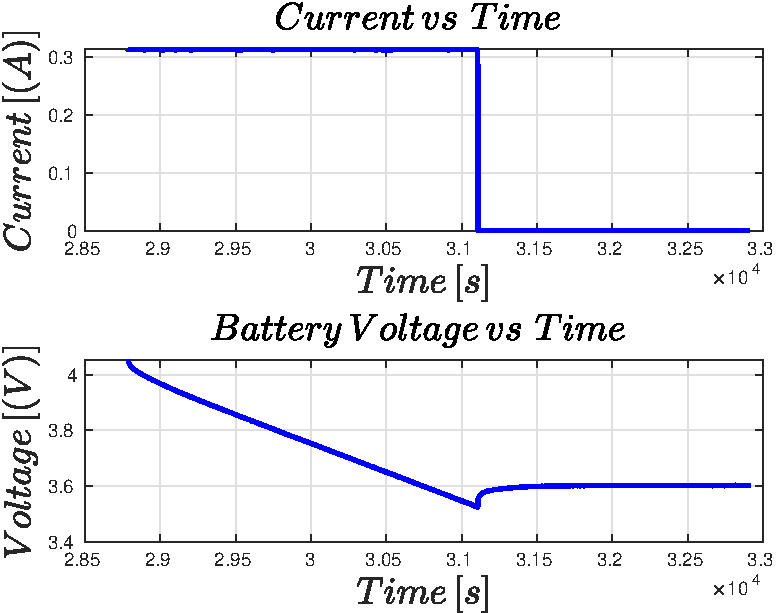
\includegraphics[width=0.8\textwidth, keepaspectratio]{images/Parameter_Identification_Region.pdf}
	\caption{Measurements of current and voltage
from a pulse response for second order equivalent circuit parameters identification.}
	\label{fig:Response_to_discharge_pulse_experimental}
\end{figure}

\par \noindent Before starting the parameter identification, continuous time dynamic equation  in \ref{eqn:continues_time_state_space}, i.e. $\dot{\bm{x}}(t) = \bm{A}\bm{x}(t)\,+\,\bm{B}u(t)$, must be discretized. Some minor arrangement in the state vector, $\bm{x}$, state transition matrix, $\bm{A}$, and input matrix, $\bm{B}$, is made for identification. State vector consists of series RC circuit voltages, $\bm{x} = [U_{1}\,\,U_{2}]^{T}$, and state transition matrix becomes $\bm{A} = \begin{bmatrix} -\frac{1}{R_{1}C_{1}} & 0 \\ 0 & -\frac{1}{R_{2}C_{2}} \end{bmatrix}$. Input matrix denoted as $\bm{B} = \begin{bmatrix} \frac{1}{C_{1}} \\ \frac{1}{C_{2}} \end{bmatrix}$. If the state equations $\dot{\bm{x}}(t) = \bm{A}\bm{x}(t)\,+\,\bm{B}u(t)$ are rearranged, and all terms pre-multiplied by the square matrix $e^{-\bm{A}t}$:

\begin{equation}
	\label{eqn:Solution_of_state_space equation_1}
	e^{-\bm{A}t}\dot{\bm{x}}(t) - e^{-\bm{A}t}\bm{A}\bm{x}(t) = \frac{d}{dt}\bigg(e^{-\bm{A}t}\bm{x}(t)\bigg)  = e^{-\bm{A}t}\bm{B}u(t)
\end{equation}

\noindent Integration of Eq. \ref{eqn:Solution_of_state_space equation_1} gives

\begin{equation}
	\label{eqn:Solution_of_state_space equation_2}
   \int_{0}^{t}\frac{d}{d\tau}\bigg(e^{-\bm{A}\tau}\bm{x}(\tau)\bigg) d\tau = \int_{0}^{t} e^{-\bm{A}t}\bm{B}u(t) =  e^{-\bm{A}t}\bm{x}(t) - e^{-\bm{A}0}\bm{x}(0) = \int_{0}^{t} e^{-\bm{A}\tau}\bm{B}u(\tau)d\tau
\end{equation}
\noindent where $e^{-\bm{A}0} = \bm{I}$ is $2\times2$ identity matrix and $[e^{-\bm{A}t}]^{-1} = e^{\bm{A}t}$ the complete state vector response may be written in two similar forms

\begin{subequations} 
	\label{eqn:Solution_of_state_space equation_3}
	\begin{align} 
	 \bm{x}(t) &= e^{\bm{A}t}\bm{x}(0)  + e^{\bm{A}t}\int_{0}^{t} e^{-\bm{A}\tau}\bm{B}u(\tau)d\tau\\
	 \bm{x}(t) &= e^{\bm{A}t}\bm{x}(0)  + \int_{0}^{t} e^{\bm{A}(t-\tau)}\bm{B}u(\tau)d\tau
	\end{align} 
\end{subequations}

\noindent A continuous time signal $\{x(t)\}$ can be obtained from a discrete time (DT) signal ${x[k]}$, by holding the value of the DT signal constant for one sampling period $T$ or $\Delta t$, such that:

\begin{equation}
	\label{eqn:zero_order_hold}
	{x}(t) = x[k], \;\;\; kT \leq t < (k+1)T
\end{equation}
This is known as the \text{zero-order hold}. The discrete-time equivalent of equation \ref{eqn:continues_time_state_space} is of the form:

\begin{align}
	\begin{split}
	\bm{x}[k+1] &= \bm{A_{d}}\bm{x}[k] + \bm{B_{d}}u[k] \\
		y[k] &= \bm{C_{d}}\bm{x}[k] +  D_{d}u[k]
	\end{split}
\end{align}

\noindent Starting from the solution of the continuous state-space equation \ref{eqn:Solution_of_state_space equation_3}, that the corresponding discrete matrices are obtained as: 

\begin{equation}
	\label{eqn:discrete_system_matrices}
	\bm{A_d} = e^{\bm{A}T}\;\;\;\text{and}\;\;\;\bm{B_{d}}=\bigg(\int_{0}^{T}e^{A\tau}d\tau\bigg)\bm{B} 
\end{equation}

\noindent It should be note that that this is the \textit{exact} solution to the differential equation, there are no discretization errors. While it is exact, information is still lost by the discretization: the inter-sample behavior. So discrete time dynamic equation can be explicity written as follows:

\begin{equation}
	\label{eqn:discrete_state_space_matrix_form}
	\bm{x}[k+1] = \underbrace{\begin{bmatrix}
		e^{-\frac{Tt}{\tau_{1}}} & 0 \\
		0 & e^{-\frac{T}{\tau_{2}}} 
	\end{bmatrix}}_{\let\scriptstyle\textstyle\substack{\bm{A}_{d}}} \bm{x}[k] + \underbrace{\begin{bmatrix}
	R_{1}(1 - e^{\frac{T}{\tau_{1}}})  \\
	R_{2}(1 - e^{\frac{T}{\tau_{2}}})  
\end{bmatrix}}_{\let\scriptstyle\textstyle\substack{\bm{B}_{d}}} u[k]
\end{equation}

\noindent where state vector is of the form $\bm{x}[k] = \big[U_{1}[k]\,\,U_{2}[k]\big]^{T}$, and input $u[k]$ is the measured current at each sampling time $I[k]$. And the continuous time matrices $\bm{C} = \bm{C_{d}}$ and $D=D_{d}$ remain same in discrete time. The discretized equations of the second order RC model may also expressed as:

\begin{align}
	\label{eqn:discrete_state_space_equation_form}
	\begin{split}
		&U_{1}[k+1] = U_{1}[k]e^{-\frac{T}{\tau_{1}}} + I[k] R_{1}\big(1 - e^{\frac{T}{\tau_{1}}}\big) \\
		&U_{2}[k+1] = U_{2}[k]e^{-\frac{T}{\tau_{2}}} + I[k] R_{2}\big(1 - e^{\frac{T}{\tau_{2}}}\big)\\ 
		&U_{t}[k] = U_{OC}\big[SOC[k]\big] - I[k] R_{0} - U_{1}[k] - U_{2}[k]
	\end{split}
\end{align}

\subsection{Parameter Identification Procedure}
To identify the parameters of the given battery model as $\bm{\Theta} = [R_{0}\,\,R_{1}\,\,\tau_{1}\,\,R_{2}\,\,\tau_{2}]^{T}$, the sum of squares
errors of the measured terminal voltage data denoted as $U_{t}^{exp}$ and the simulated terminal voltage data denoted as $U_{t}^{sim}$ for the terminal
voltage at each sampling point of input current is chosen as the objective function, which is represented
by the summation of square of the $\ell_{2}-norm$ or $Euclidean\,norm$, ${\norm x}_{2}^{2}$ as follows:  

\begin{equation} 
	\label{eqn:optimization_problem_formulation}
	\begin{aligned}
		& \underset{\bm{\Theta}}{\text{min}}
		& & \bm{\textit{J}}(\bm{\Theta},k) = \underset{\bm{\Theta}}{\text{min}} \sum_{k=k_{0}}^{N}\bigg(U_{t}^{exp}[k] - U_{t}^{sim}[\bm{\Theta},k]\bigg)^{2} \\
		& \text{st.}
		& & \bm{\Theta}_{i} \geq 0, \;\;i = 1, \dots, 5 \\
		& 
		& & \bm{x}[k+1] = \bm{A}_{d}\bm{x}[k] + \bm{B}_{d}u[k],\;\; k = k_{0},\dots,N-1\\
		& 
		& & U_{t}^{sim}[k] = U_{OC}\big[SOC[k]\big] + \bm{C}_{d}x[k] + D_{d}u[k],\,\, k = k_{0},\dots,N 
	\end{aligned} 
\end{equation}
where $k_{0}$ is starting time and $N$ is the final time of the identification process, input is the measurement current, $I[k]=u[k]$ in the input current and $\bm{\Theta}$ is the identified parameter vector. 
\href{https://www.mathworks.com/videos/automating-the-parameter-estimation-of-a-battery-model-95187.html}{(Some ready-to-run implementation is also available for parameter estimation in MATLAB.)} Initial value of the state vector is accepted is zero, $\bm{x}[k=k_{0}]=\bm{0}$, because of the fact that battery is at the idle state before the parameter estimation procedure. \newline 

\par \noindent [\textbf{NOTE}]: \textbf{Solution of this optimization technique is postponed. Particle Swarm Optimization (PSO) technique will be considered for solution.}

\subsection{Parameter Identification Based On Recursive Least Square (RLS)\cite{Fazheng2019}} 
From equation \ref{eqn:electrical_behavior_of_the_proposed_model}, the transfer function of the second-order equivalent circuit model
can be written as:

\begin{equation}
	\label{eqn:transfer_function_Laplace_domain}
	G(s) = \frac{U_t(s) - U_{oc}(s)}{I(s)} = -\bigg(R_{0} + \frac{R_{1}}{1+\tau_{1}s} + \frac{R_{2}}{1+\tau_{2}s} \bigg)
\end{equation}

\noindent Then, the transfer function is transformed from $\mathcal{L}$ (Laplace) domain to $z$ domain based on \href{https://tttapa.github.io/Pages/Mathematics/Systems-and-Control-Theory/Digital-filters/Discretization/Bilinear-transform.html#:~:text=The%20bilinear%20transform%20is%20a,trapezoidal%20rule%20for%20numerical%20integration}{bilinear transformation}, which can be expressed as:

\begin{equation}
	\label{eqn:bilinear_transformation}
	s = \frac{2(1-z^{-1})}{T(1+z^{-1})}
\end{equation}

\noindent where $T$ is the sampling time of the system. Substituting Equation \ref{eqn:transfer_function_Laplace_domain} for \ref{eqn:bilinear_transformation}, the discrete transfer function of the system can be
written as:

\begin{equation}
	\label{eqn:transfer_function_z_domain}
	G(z^{-1}) = \frac{\theta_{3} + \theta_{4}z^{-1} + \theta_{5}z^{-2}}{1-\theta_{1}z^{-1}-\theta_{2}z^{-2}}
\end{equation}

\noindent where parameters $\theta_{i} (i = 1, 2, ..., 5)$ can be identified by recursive least square method. The relation between RLS parameters and equivalent circuit RC parameters are explained in Appendix \ref{Relation_RLS_Parameter_Circuit_Parameter} in detail. The RC parameters of the circuit can be obtained by the following equations. Let $y[k] = U_{t}[k] - U_{oc}[k]$, Equation \ref{eqn:transfer_function_z_domain} can be written as follows:

\begin{equation}
	\label{eqn:discrete_output_equation}
	y[k] = \theta_{1}y[k-1] + \theta_{2}y[k-1] + \theta_{3}I[k] + \theta_{4}I[k-1] + \theta_{5}I[k-2]
\end{equation}

\noindent Defining $\bm{\phi}$ and new parameter vector, $\bm{\theta}$ as,

\begin{equation}
	\label{eqn:RLS_psi_vector}
	\bm{\phi}[k] = \bigg[y[k-1]\,\,y[k-2]\,\,I[k]\,\,I[k-1]\,\,I[k-2]\bigg]^{T} 
\end{equation}

\begin{equation}
	\label{eqn:RLS_theta_vector}
	\bm{\theta}[k] = \big[\theta_{1}\,\,\theta_{2}\,\,\theta_{3}\,\,\theta_{4}\,\,\theta_{5}\big]^{T} 
\end{equation}

\noindent Then Equation \ref{eqn:discrete_output_equation} can be written in vector form as follows:

\begin{equation}
	\label{eqn:discrete_output_equation_2}
	y[k] = \bm{\phi}[k]^{T}\bm{\theta}[k]
\end{equation}

\noindent Defining the estimator of $\bm{\theta}$ as $\bm{\hat{\theta}}$, Equation \ref{eqn:discrete_output_equation_2} can be expressed as:

\begin{equation}
	\label{eqn:discrete_output_equation_3}
	y[k] = \bm{\phi}[k]^{T}\bm{\hat{\theta}}[k] + \varepsilon[k]
\end{equation}	

\noindent When the square sum of $\varepsilon$ the output error is minimum, the parameters are optimal, and the mathematical formula
can be written as:

\begin{equation}
	\label{eqn:RLS}
	\underset{\bm{\hat{\theta}}}{\text{min}} \,\,\bm{\textit{J}}(\bm{\hat{\theta}},k) = \underset{\bm{\hat{\theta}}}{\text{min}} \sum_{k=k_{0}}^{N}\varepsilon[k]^{2} = \underset{\bm{\hat{\theta}}}{\text{min}} \sum_{k=k_{0}}^{N}\bigg(y[k] - \bm{\phi}[k]^{T}\bm{\hat{\theta}}[k]\bigg)^{2}
\end{equation}

\noindent Taking the derivation of $\bm{\hat{\theta}}$ with respect to $\bm{\theta}$ and then equal to zero, the solution can be obtained:

\begin{equation}
	\label{eqn:Least_square_one_step_solution}
	\bm{\hat{\theta}} = (\bm{\Psi}^{T}\bm{\Psi})^{-1}\bm{\Psi}^{T}\bm{Y}
\end{equation}
where vectors compose of past measurements $\bm{\Psi}= \big[\bm{\phi}[k_{0}]\,\,\bm{\phi}[k_{0}+1]\,\,\dots\,\,\bm{\phi}[N]\big]^{T}$ and big output vector $\bm{Y}=\big[y[k_{0}]\,\,y[k_{0}+1]\,\,\dots\,\,y[N]\big]^{T}$. Step of the RLS algorithm is explained following chapter.

\subsubsection{The Parameter Estimation Algorithm}
The algorithm for recursive least squares estimation is summarized as follows.

\begin{itemize}
	\item Initialize the estimator:
	
	\begin{align}
	\label{eqn:RLS_Algorithm_01}
	\begin{split}
	& \bm{\hat{\theta}}[k_{0}] = E\big[\bm{\theta}[k_{0}]\big] \\
	& \bm{P}[k_{0}] = E\bigg[\big(\bm{\theta}[k_{0}]-\bm{\hat{\theta}}[k_{0}])(\bm{\theta}[k_{0}]-\bm{\hat{\theta}}[k_{0}]\big)^{T}\bigg]
	\end{split}
	\end{align}
	
	In the case of no prior knowledge about $\bm{\theta}[k_{0}]$, simply let $\bm{P}[k_{0}]=\infty \bm{I}$. In the case of perfect prior knowledge, let $\bm{P}[k_0] = 0$.
	
	\item Update the estimate $\bm{\hat{\theta}}[k]$ and the covariance of the estimation error sequentially, which are listed below:
	
	\begin{subequations} 
		\label{eqn:RLS_equations}
		\begin{align} \bm{K}[k] &= \bm{P}[k-1]\,\bm{\phi}[k]\big(\bm{\phi}[k]^{T}\bm{P}[k-1]\bm{\phi}[k]+1\big)^{-1} \\ 
		\bm{P}[k] &= \big(\bm{I} - \bm{K}[k]\bm{\phi}[k]^{T}\big)\bm{P}[k-1] \\
		\bm{\hat{\theta}}[k] &= \bm{\hat{\theta}}[k-1] + \bm{K}[k]\big(y[k]-\bm{\phi}[k]^{T}\bm{\hat{\theta}}[k-1]) 
		\end{align} 
	\end{subequations} 
	
\end{itemize}

\lstinputlisting{MATLAB_Files/Recurcive_Least_Square.m} 

\noindent Parameter identification results of  least square algorithm is given in the Fig . As it can be seen in subplots, some parameters of the equivalent circuit element is found in negative. The main reason of this observation is thought that OCV-SOC relation is inadequately obtained.  

\begin{figure}[t!]
	\centering
	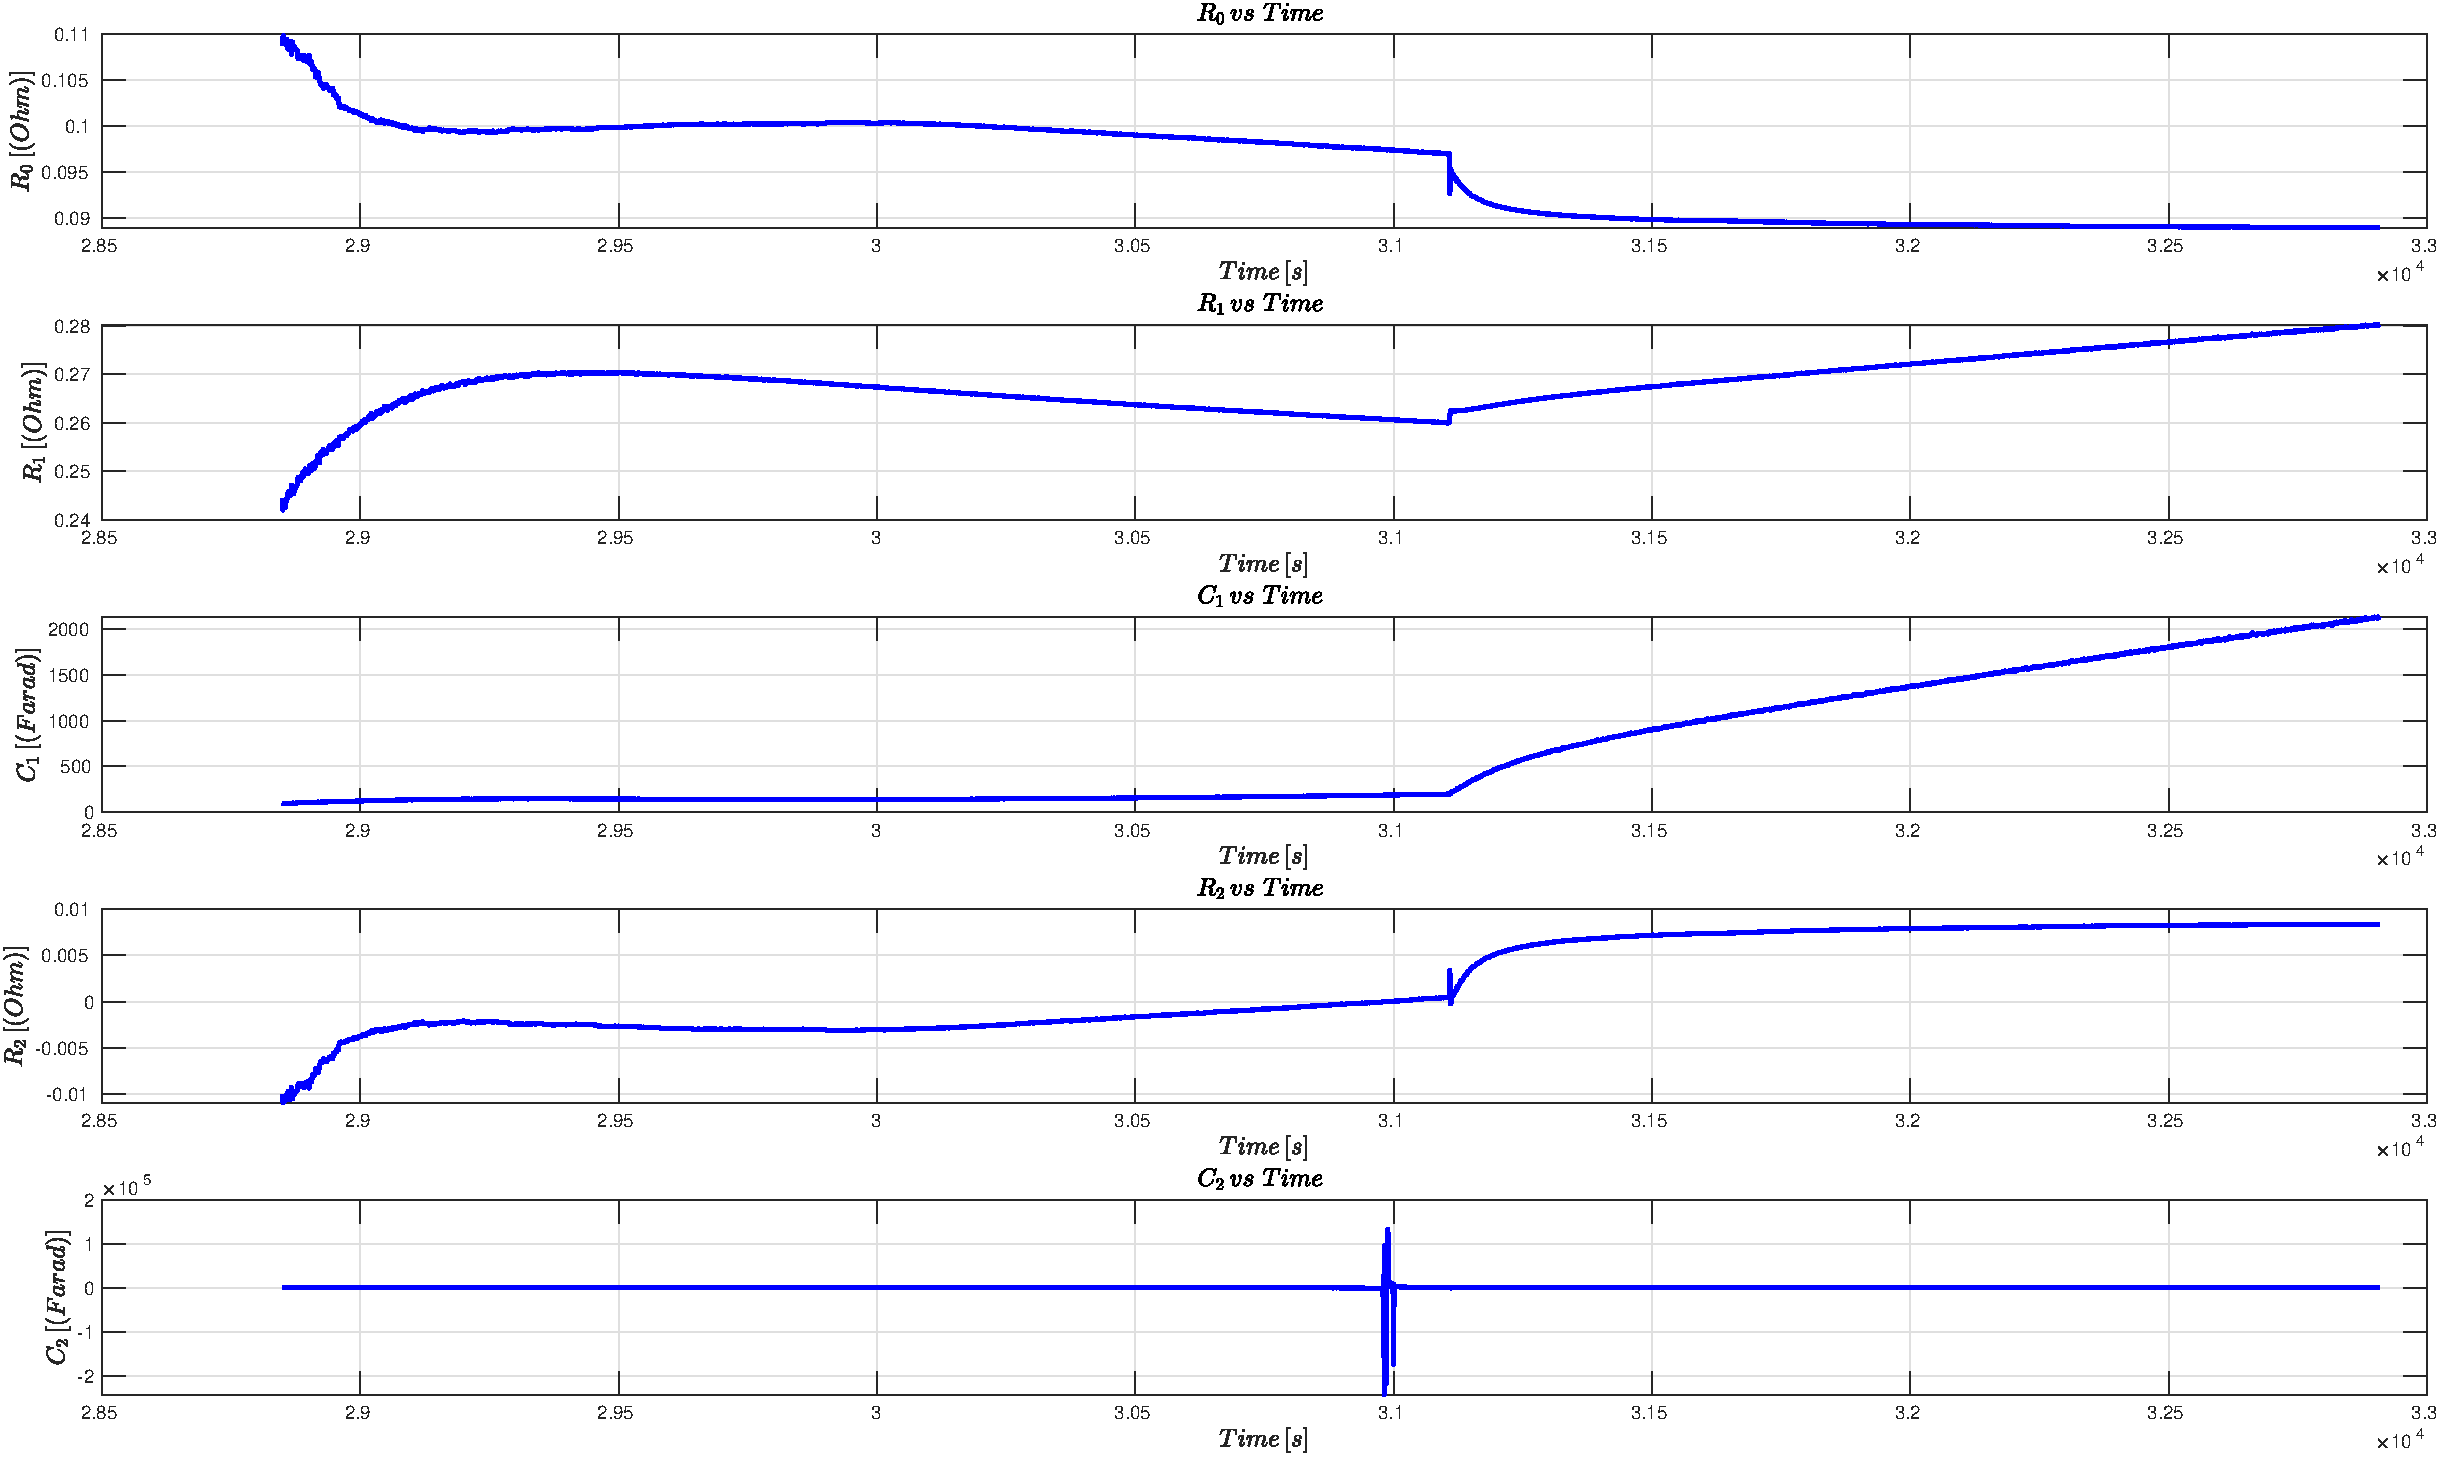
\includegraphics[width=\textwidth, keepaspectratio]{images/RLS_Results.pdf}
	\caption{Parameter identification results of the RLS algorithm for parameters $R_{0}$, $R_{1}$, $R_{2}$, $C_{1}$ and $C_{2}$.}
	\label{fig:Results_of_the_RLS_Method}
\end{figure}

\section{SOC Estimation Method Based on the Adaptive EKF \cite{Pang2018}} 
\label{SOC_Estimation_Based_on_the_Adaptive_EKF}

The adaptive extended Kalman filter is used to make the SOC estimation because the covariance
 parameters in AEKF approach are not taken as constant, but adaptively updated online with
a dedicated SOC estimator which can enhance the estimation performance with respect
to the EKF. The control input of the SOC estimator is the current representing the behavior of the battery during discharge or charge process, the output the SOC
estimator is the SOC value estimated by the AEKF algorithm.

\subsection{AEKF Algorithm}
\label{Adaptive_EKF}

Extended Kalman filter's performance is strongly dependent on the accuracy of the predetermined noise matrix. Thus, it is necessary for the AEKF algorithm to adopt this problem in battery applications. To apply the AEKF for the SOC estimation, it is necessary to reform a state-space form as shown in Equation \ref{eqn:discrete_state_space_matrix_form}. Discrete-time SOC equation \ref{eqn:SOC_in_discrete_time} is also written as a dynamic equation and new state space representation becomes: 

\begin{figure}[t!]
	\centering
	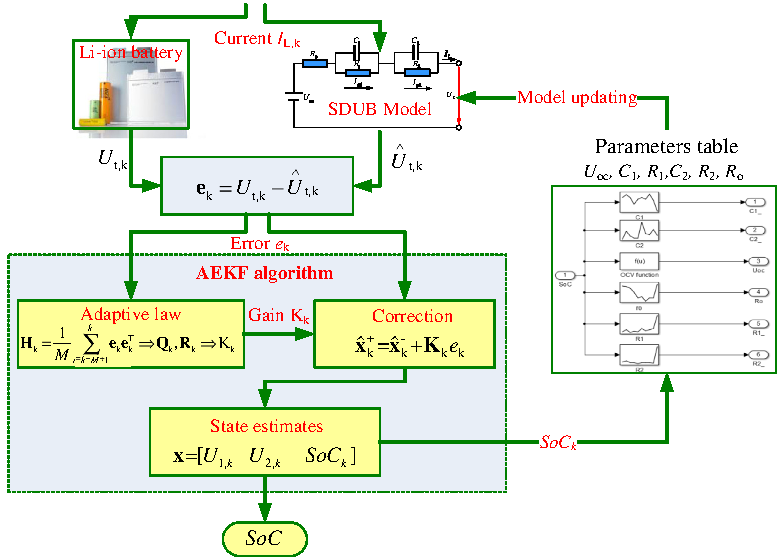
\includegraphics[width=0.6\textwidth, keepaspectratio]{images/Data_Driven_SoC_Estimation_Approach_With_AEKF_Algorithm.pdf}
	\caption{The implementation flowchart of the data driven-based SoC estimation approach with AEKF algorithm. \cite{Xiong2013}}
	\label{fig:AEKF_Algorithm_Flowchart}
\end{figure}

\begin{align}
	\label{eqn:discrete_state_space_matrix_form_for_EKF_1}
	\begin{split}
		\bm{x}[k+1] &= f(\bm{x[k]},u[k]) =\bm{A_{d}}\bm{x}[k] + \bm{B_{d}}u[k] + \bm{w}[k]\\
		y[k] &= h(\bm{x[k]},u[k]) + v[k]
	\end{split}
\end{align}

\noindent Explicity,

\begin{equation}
	\label{eqn:discrete_state_space_matrix_form_for_EKF_2}
	\bm{x}[k+1] = \underbrace{\begin{bmatrix}
			e^{-\frac{Tt}{\tau_{1}}} & 0 & 0\\
			0 & e^{-\frac{T}{\tau_{2}}} & 0 \\
			0 & 0 & 1
	\end{bmatrix}}_{\let\scriptstyle\textstyle\substack{\bm{A}_{d}}} \bm{x}[k] + \underbrace{\begin{bmatrix}
			R_{1}(1 - e^{\frac{T}{\tau_{1}}})  \\
			R_{2}(1 - e^{\frac{T}{\tau_{2}}})  \\
			-\frac{\eta T}{Q}
	\end{bmatrix}}_{\let\scriptstyle\textstyle\substack{\bm{B}_{d}}} u[k]
	+ \bm{w}[k]
\end{equation}

\noindent The output equation is the same as it used to be \ref{eqn:discrete_state_space_equation_form}. The state vector with SOC is denoted by $\bm{x}[k] = \bigg[U_{1}[k]\,\,U_{2}[k]\,\,SOC[k]\bigg]^{T}$. $\bm{w}[k]$ is the unmeasured process noise that
affects the system state and $v[k]$ is the measurement noise which does not affect the system state, but can be reflected in the system
output estimation $y[k]$. $\bm{w}[k] \sim \mathcal{N}(0,\,\bm{Q})$ is assumed to be Gaussian white noise with zero mean and covariance $\bm{Q}[k]$; $v[k] \sim \mathcal{N}(0,\,\bm{R})$ is assumed to be Gaussian white noise with zero mean and covariance $R[k]$. The AEKF provides a further innovation using the filter’s innovation sequence and the innovation allows the parameters $\bm{Q}$ and $R$ to be estimated and updated iteratively. \newline 

\par \noindent The matrix $\bm{C}$ that is employed in the AEKF filter is the derivative of the output equation \ref{eqn:discrete_state_space_matrix_form_for_EKF_1} with respect to state vector before estimation time, i.e. $\bm{C}[k]= \dfrac{\partial h(\bm{x}[k],u[k])}{\partial \bm{x}}\Biggr|_{\substack{x=\hat{x}[k]^{-}}} = \bigg[-1\,-1\,\dfrac{dU_{oc}(SOC)}{dSOC}\Bigr|_{\substack{\hat{SOC}[k]^{-}}}\bigg]$. As it can be seen in $C$ matrix, the derivation of the OCV-SOC model function, $\dfrac{dU_{oc}(SOC)}{dSOC} = K_{1}SOC^{-2}-K_{2}+ \dfrac{K_{3}}{SOC}-\dfrac{K_{4}}{1-SOC}$ is utilized from the second row of Table \ref{table:Comparing_Fitting_Results}. The AEKF Algorithm is explained in the following Algorithm \ref{Alg:The_AEKF_Algorithm} by using above equations and relations. 

\begin{algorithm}
	\caption{The AEKF Algorithm \label{Alg:The_AEKF_Algorithm}}
	\DontPrintSemicolon	
	\KwInput{$u[k]=I[k], ~k \in\{k_{0},\dots\,N-1\}$}
	\KwOutput{$\widehat{SOC}[k],~k \in\{k_{0},\dots\,N-1\}$}
	\KwData{$y[k] = U_{t}^{exp}[k],~k \in \{k_{0},\dots\,N\}$,~$R_{0}[k]$,~$R_{1}[k]$,~$C_1[k]$,~$R_{2}[k]$,~$C_{2}[k]$}
	\nonl$\textbf{Step 1: Initialization:}$\\
	\nonl$\bm{\hat{x}}[k_{0}-1]^{+} = E\big[\bm{x}[k_{0}-1]\big]$,~$\bm{\hat{P}}[k_{0}-1]^{+}=E\bigg[\bigg(\bm{x}[k_{0}-1]-E\big[\bm{\hat{x}}[k_{0}-1]^{+}\big]\bigg)\bigg(\bm{x}[k_{0}-1]-E\big[\bm{\hat{x}}[k_{0}-1]^{+}\big]\bigg)^{T}\bigg]$\\
	\nonl$\textbf{Step 2: Calculation:}$\\
	\nonl\For{$k = k_{0} \to N$} 
	{
		\textbf{State Estimation Propagation:} $\bm{\hat{x}}[k]^{-} = f\bigg(\bm{\hat{x}}[k-1]^{+},u[k]\bigg)$ ~(look \ref{eqn:discrete_state_space_matrix_form_for_EKF_1})\\
		\vspace{3mm}
		
		\textbf{State Estimation Covariance:} $\bm{P}[k]^{-} = \bm{A_{d}}[k]\bm{P}[k-1]\bm{A_{d}}[k]^{T} + \bm{Q}[k-1]$ \\
		\vspace{3mm}
		
		\textbf{Error Innovation:} $e[k] = y[k]-h\bigg(\bm{\hat{x}}[k]^{-},u[k]\bigg)$ \\
		\vspace{3mm}
		
		\textbf{Adaptive Law:} $H[k] = \dfrac{1}{M}\sum_{i=k-M+1}^{k}e[k]^2$,~$R[k]=H[k]-\bm{C}[k]\bm{P}[k]^{-}\bm{C}[k]^{T}$ \\
		\vspace{3mm}
		
		\textbf{Kalman Gain Matrix:} $\bm{K}[k] = \bm{P}[k]^{-}\bm{C}[k]^{T}\bigg(\bm{C}[k]\bm{P}[k]^{-}\bm{C}[k]^{T}+R[k]\bigg)^{-1}$ 
		\vspace{3mm}
		
		\textbf{State Estimate Measurement Update:} $\bm{\hat{x}}[k]^{+} = \bm{\hat{x}}[k]^{-} + \bm{K}[k]e[k]$  \\
		\vspace{3mm}
		
		\textbf{State Covariance Measurement Update:} $\bm{Q}[k] = \bm{K}[k]H[k]\bm{K}[k]^{T}$, ~$\bm{P}[k]^{+} = \bigg(\bm{I}-\bm{K}[k]\bm{C}[k]\bigg)\bm{P}[k]^{-}\bigg(\bm{I}-\bm{K}[k]\bm{C}[k]\bigg)^{T} + \bm{K}[k]\bm{R}[k]\bm{K}[k]^{T}$ \\
		 \vspace{3mm}
		 
		\tcc*{$\bm{A}_{d}[k]= \dfrac{\partial f(\bm{x}[k],u[k])}{\partial \bm{x}}\Biggr|_{\substack{x=\hat{x}[k]^{-}}}$,~$\bm{C}[k]= \dfrac{\partial h(\bm{x}[k],u[k])}{\partial \bm{x}}\Biggr|_{\substack{x=\hat{x}[k]^{-}}}$} 
	}

\end{algorithm}


\begin{figure}[t!]
	\centering
	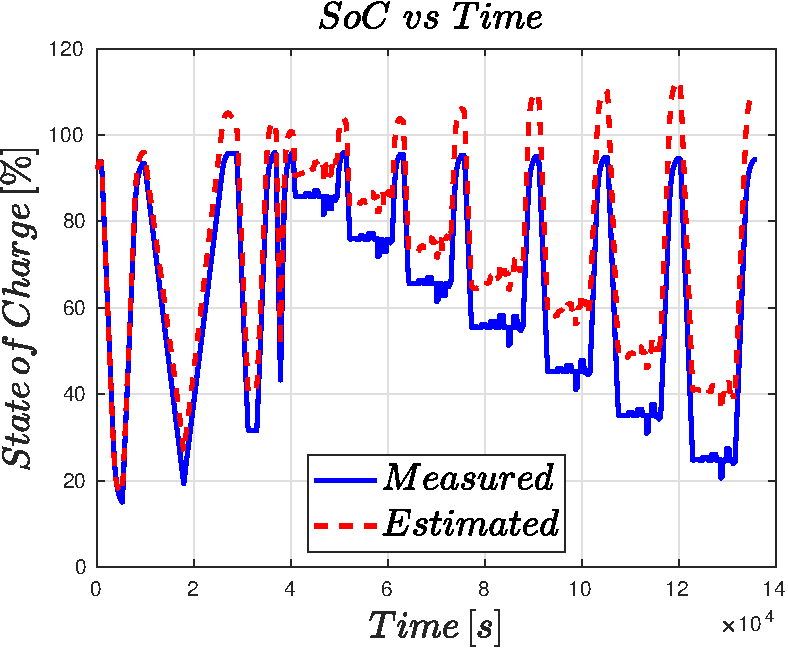
\includegraphics[width=0.7\textwidth, keepaspectratio]{images/AEKF_SOC.pdf}
	\caption{Validation results for SOC estimation by using AEKF.}
	\label{fig:The_AEKF_SOC}
\end{figure}

\begin{figure}[b!]
	\centering
	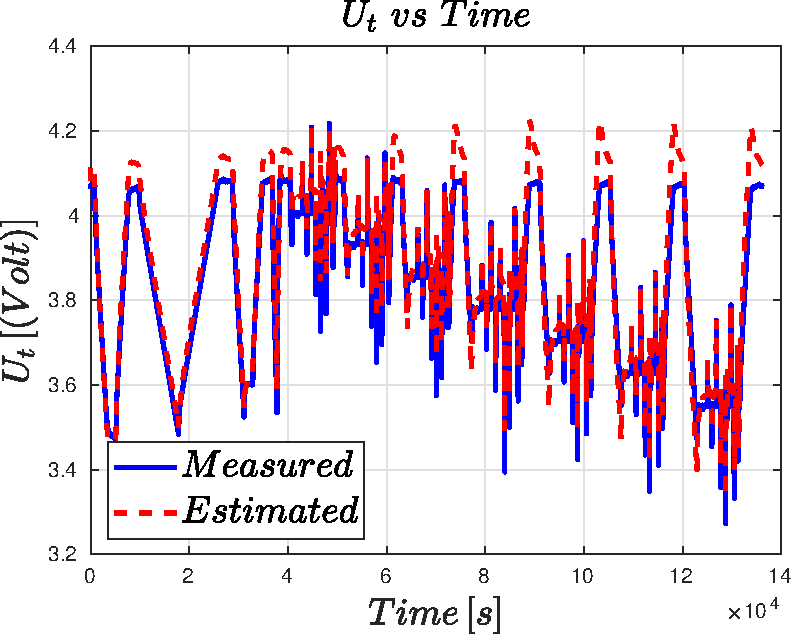
\includegraphics[width=0.7\textwidth, keepaspectratio]{images/AEKF_Terminal_Voltage.pdf}
	\caption{Validation results for terminal voltage, $U_{t}$, by using AEKF}
	\label{fig:The_AEKF_Terminal_Voltage}
\end{figure}

\par \noindent It should be pointed out that $\bm{\hat{x}}[k]^{-}$ and $\bm{\hat{x}}[k]^{+}$ are both estimations of the same vector $\bm{x}[k]$. However,$\bm{\hat{x}}[k]^{-}$ is the estimate of $\bm{\hat{x}}[k]$ before the measurement $y[k]$ is considered, which is called the a priori estimate, and $\bm{\hat{x}}[k]^{+}$ is the estimate of $\bm{x}[k]$ after the measurement $y[k]$ is taken into account, which is called the a posteriori estimate.  The voltage error $e[k]$ is computed and the adaptive law $\bm{H}[k]$ is employed to update $\bm{\hat{x}}[k]$, $\bm{P}[k]$, $\bm{Q}[k]$ and $\bm{K}[k]$. Then, the updated gain is used to
compensate for the state estimation error. The SOC estimation is fed back to update the parameters of the battery model for the SOC estimation at the next sampling time. Implementation of the AEKF is at Appendix,. In the simulation study, \textit{Adaptive Law} is skipped due to the high values coming from $\bm{C}[k]\bm{P}[k]^{-}\bm{C}[k]^{T}$. So that, $R[k]$ taken as constant during the simulation. The following figures show the results of the AEKF, actually EKF, technique. 


\begin{figure}[h!]
	\centering
	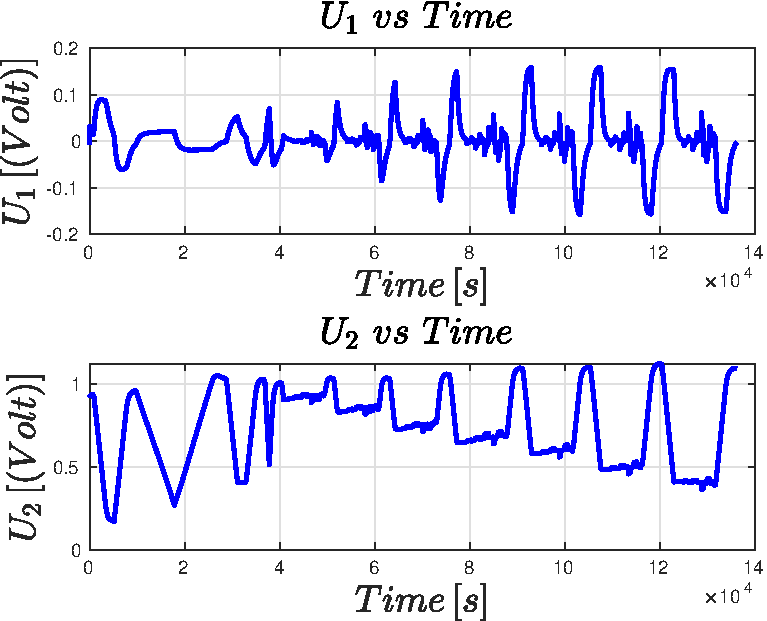
\includegraphics[width=0.7\textwidth, keepaspectratio]{images/AEKF_RC_Voltages.pdf}
	\caption{AEKF's state estimation for RC voltages $U_{1}$ and $U_{2}$, respectively }
	\label{fig:The_AEKF_RC_Voltages}
\end{figure}

\begin{figure}[h!]
	\centering
	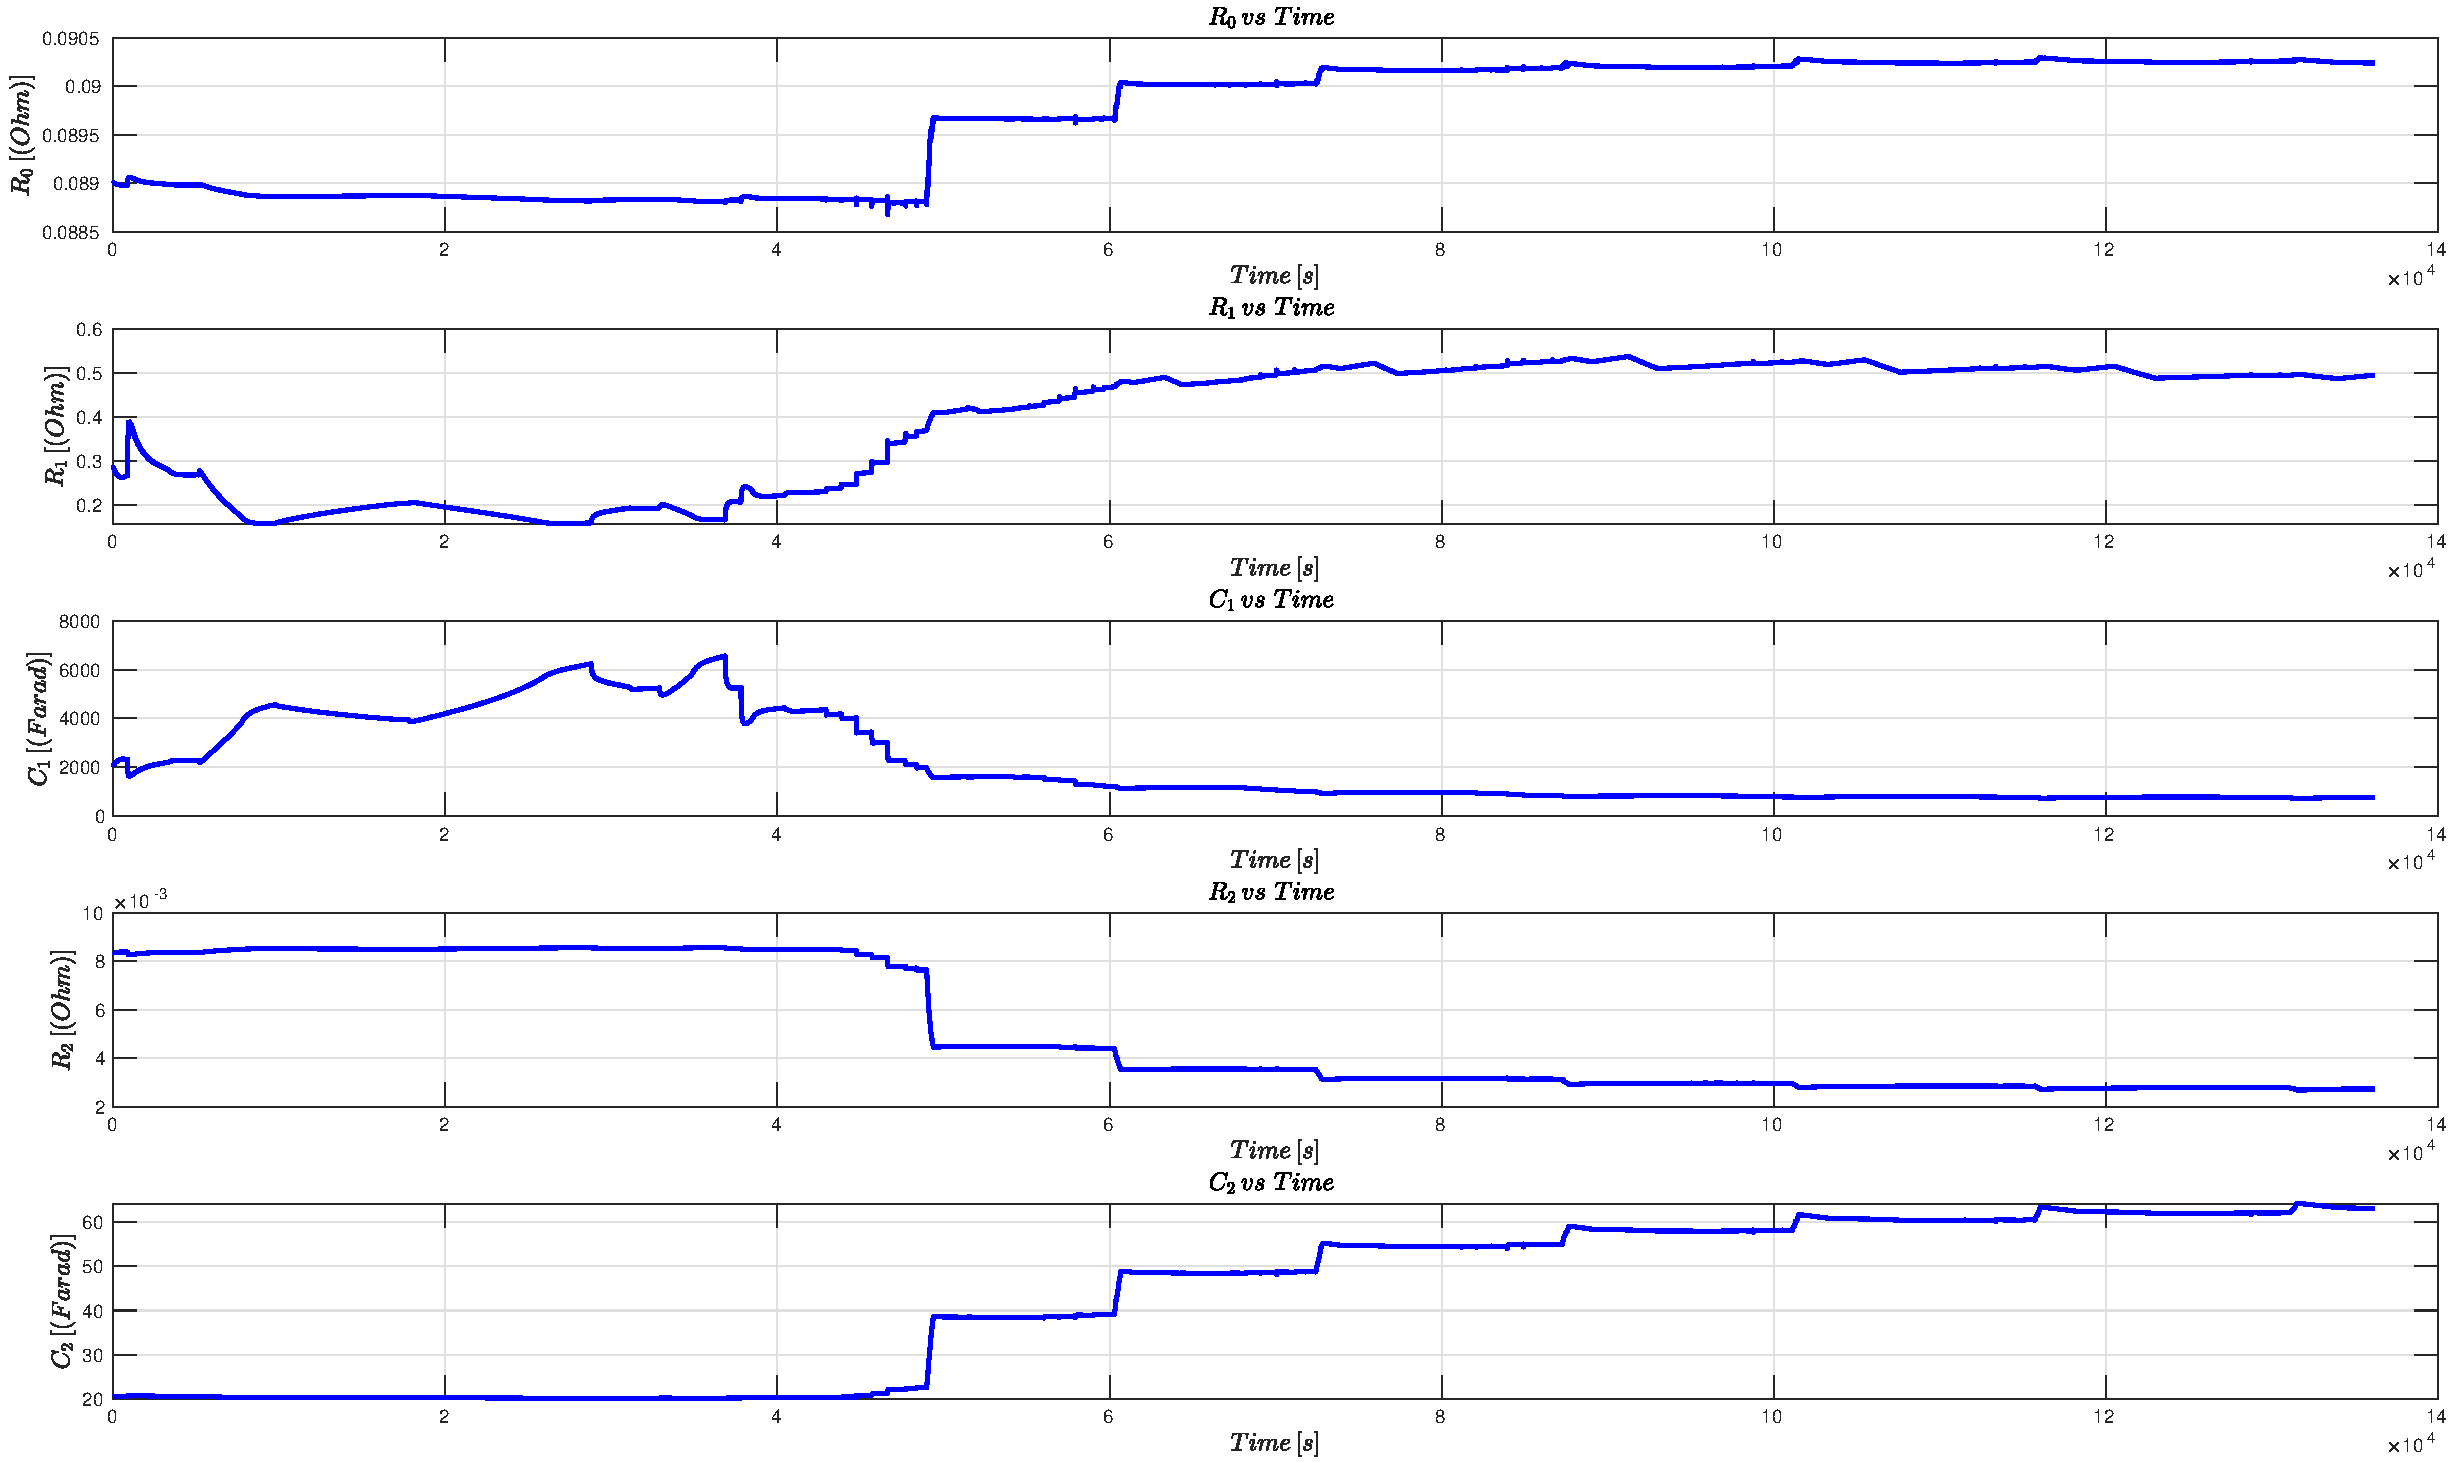
\includegraphics[width=1.0\textwidth, keepaspectratio]{images/RLS_Results_With_AEKF.pdf}
	\caption{Estimated Parameters by using RLS through whole experiment time.}
	\label{fig:RLS_Results_With_AEKF}
\end{figure}


\clearpage
\bibliography{references}
% You can use full name of authors, however most likely some of the Bibtex entries you will find, will use abbreviated first names
% If you don't want to correct each of them by hand, you can use abbreviated style for all of the references
\bibliographystyle{abbrv}
\clearpage

\begin{appendices}
\section{Curve Fitting for OCV Models} \label{Curve_Fitting_Appendeix}

\subsection{Model-1} \label{Model-1}
The first proposed generalized SOC-OCV model is shown in Equation \ref{eqn:OCV_SOC_Model_1}, where a logarithmic function with real (not complex) power, a linear function, and an exponential function with a shifted exponent can clearly be seen:

\begin{equation}
	\label{eqn:OCV_SOC_Model_1}
	U_{OC}(SOC(t)) = a  + b \times (-ln(SOC(t)))^m + c \times SOC(t) + d \times \exp^{n(SOC(t)-1)}
\end{equation}

\noindent where $U_{OC}$ and $s$ represent the OCV and SOC of the battery, respectively, and $0 \leq s \leq 1$, $m > 0$ and $n > 0$. The logarithmic function must be tuned to play a predominant role at low SOC, where charge accumulations on the surfaces of the active materials happen within the lithium-ion batteries. The linear function, in turn, dominates the middle SOC range, where primary phase transformation of the active materials occurs. The last exponential function then contributes to the high SOC behavior, where both partial redox reaction and charge accumulation occur. The three functions in Equation \ref{eqn:OCV_SOC_Model_1} are therefore essential, and will interact with each other to form the generalized OCV model over the whole SOC range \cite{Zhang2016}.  \newline 

\begin{figure}[b!]
	\centering
	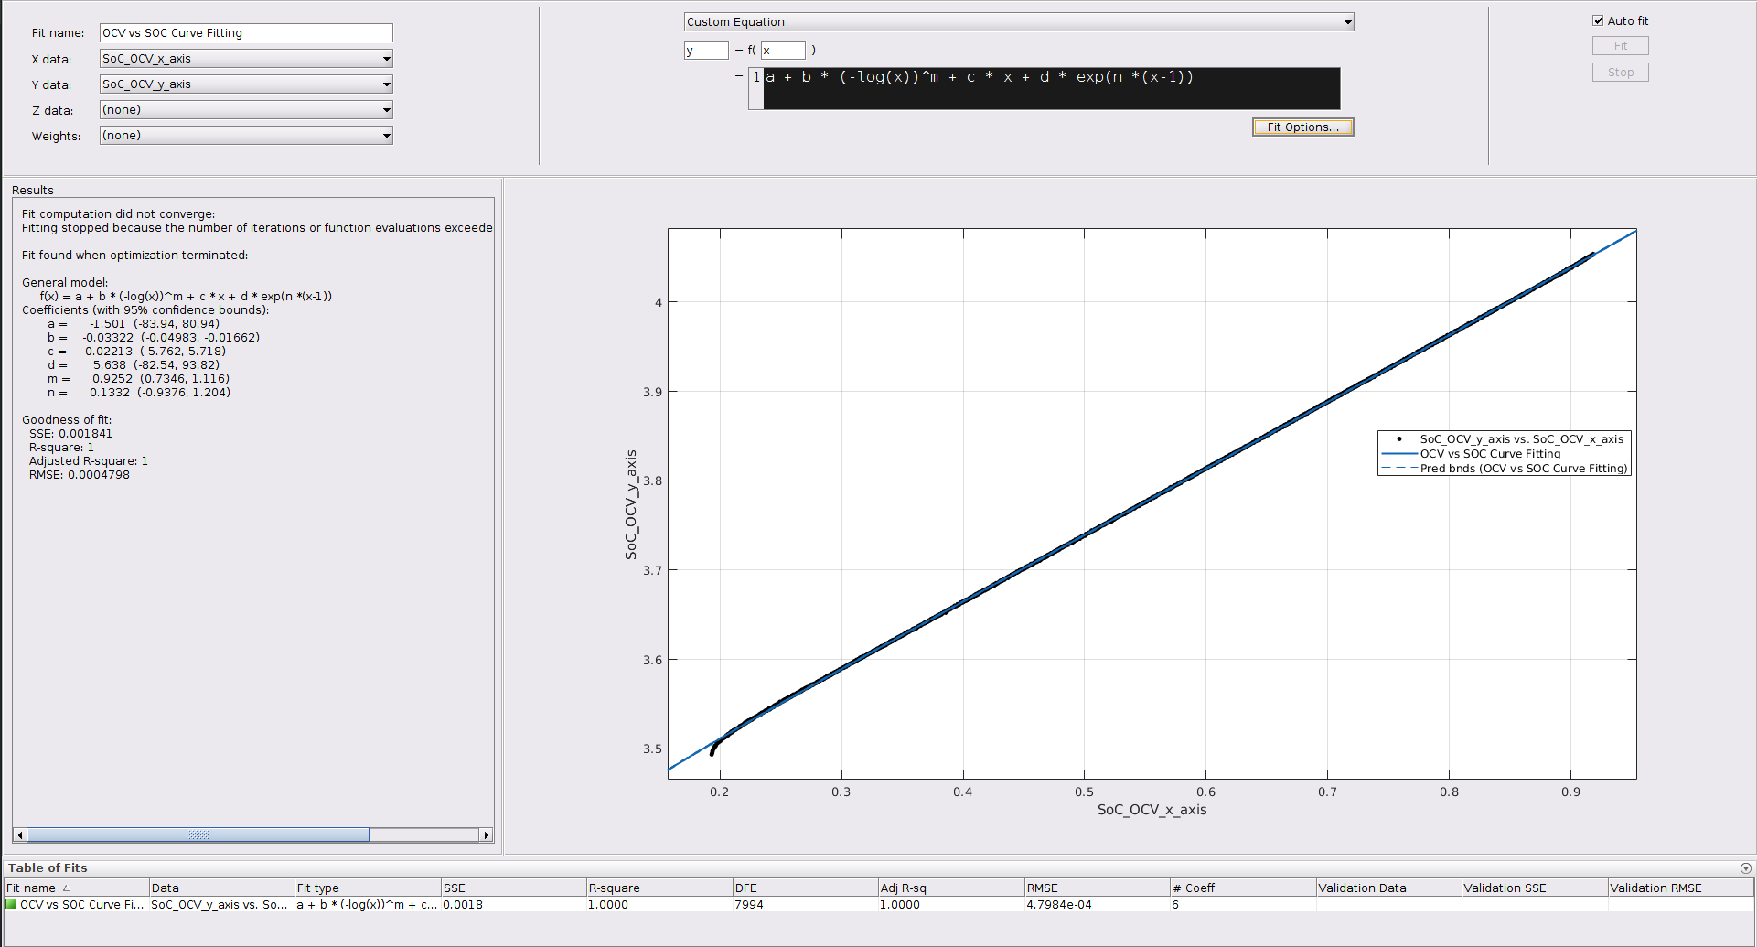
\includegraphics[width=1.0\textwidth, keepaspectratio]{images/Curve_Fitting_1.pdf}
	\caption{MATLAB Curve Fitting Toolbox for Model - 1}
	\label{fig:OCV_SOC_Model_1}
\end{figure}

\par \noindent Parameters of the function is found via \textbf{NonlinearLeastSquare} method and \textit{Trust-Region} algorithm within the boundary of the $m$ and $n$ values. Coefficients is calculated with 95\% confidence bounds. Table \ref{table:OCV_SOC_Model_1_1} shows the coefficient values and their limits and next Table \ref{table:OCV_SOC_Model_1_2} includes the sum of the squared prediction errors (SSE), the root mean square error (RMSE), R-square (i.e. it is a statistical measure of how close the data are to the fitted regression line), and adjusted R-sq.

\begin{table}[!t]
	\center
	\begin{tabular}{||c | c | c | c ||} 
		\hline
		Coefficient & Value with 95\% Confidence Bounds & Lower Bound & Upper Bound \\ [0.5ex] 
		\hline\hline
		$a$ & $-1.501$  & $-\infty$ & $\infty$ \\ 
		\hline
		$b$ & $-0.03322$ & $-\infty$ & $\infty$ \\
		\hline
		$c$ & $-0.02213$ & $-\infty$ & $\infty$ \\
		\hline
		$d$ & $5.638$ & $-\infty$ & $\infty$ \\
		\hline
		$m$ & $0.9252$ & $0$ & $\infty$ \\
		\hline
		$n$ & $0.1332$ & $0$ & $\infty$ \\
		\hline
	\end{tabular}
	\caption{\label{table:OCV_SOC_Model_1_1}Coefficients of the model-1 with bounds.}
\end{table}

\begin{table}[!t]
	\center
	\begin{tabular}{||c | c | c | c ||} 
		\hline
		SSE & RMSE & R-Square & Adjusted R-sq\\ [0.5ex] 
		\hline\hline
		$0.001841$ & $0.0004798$  & $1$ & $1$ \\ 
		\hline
	\end{tabular}
	\caption{\label{table:OCV_SOC_Model_1_2}The Goodness of fit of the model-1.}
\end{table}

\subsection{Model-2} \label{Model-2}
With SOC available as part of the model state, terminal
voltage may be predicted in a number of different ways.
Several different forms are adapted from the literature \cite{Plett2004}. \newline

\begin{tabular}{ll}
	Shepherd model:  &$U_{t}(t) = U_{OC}(SOC(t)) - R_{0}I(t) - K_{i}/SOC(t)$ \\
	Unnewehr universal model: &$U_{t}(t) = U_{OC}(SOC(t)) - R_{0}I(t) - K_{i}/SOC(t)$ \\
	Nernst model: &$U_{t}(t) = U_{OC}(SOC(t)) - R_{0}I(t) +  K_{2} ln(SOC(t))$ \\
	 &$+ K_{3}ln(1-SOC(t))$
\end{tabular} \newline

\par \noindent $K_{i}$ is
the polarization resistance and $K_{1}$, $K_{2}$ and $K_{3}$ are constants
 chosen to make the model fit the data well. All of the terms of
these models may be collected to make a “combined model”
 that performs better than any of the individual models alone.
This model is

\begin{equation}
	\label{eqn:OCV_SOC_Model_2}
	U_{t}(t) = K_{0} - R_{0}I(t) - \frac{K_{1}}{SOC(t)} - K_{2}SOC(t) + K_{3}ln(SOC(t)) + K_{4}ln(1 - SOC(t))
\end{equation}

\noindent The unknown quantities in the combined model may be estimated using a system identification procedure. This model
 has the advantage of being \textit{linear in the parameters}; that is,
the unknowns occur linearly in the output equation. From the Equation \ref{eqn:OCV_SOC_Model_2} nonlinear OCV-SOC model can be extracted as follows: 

\begin{equation}
	\label{eqn:OCV_SOC_Model_2_1}
	U_{OC}(SOC(t)) = K_{0} - \frac{K_{1}}{SOC(t)} - K_{2}SOC(t) + K_{3}ln(SOC(t)) + K_{4}ln(1 - SOC(t))
\end{equation}

\par \noindent Parameters of the above function, \ref{eqn:OCV_SOC_Model_2_1},  is found via \textbf{NonlinearLeastSquare} method and \textit{Trust-Region} algorithm within the pretty large boundary. Coefficients is calculated with 95\% confidence bounds. Table \ref{table:OCV_SOC_Model_1_1} shows the coefficient values and their limits and next Table \ref{table:OCV_SOC_Model_1_2} includes the sum of the squared prediction errors (SSE), the root mean square error (RMSE), R-square (i.e. it is a statistical measure of how close the data are to the fitted regression line), and adjusted R-sq.

\begin{figure}[t!]
	\centering
	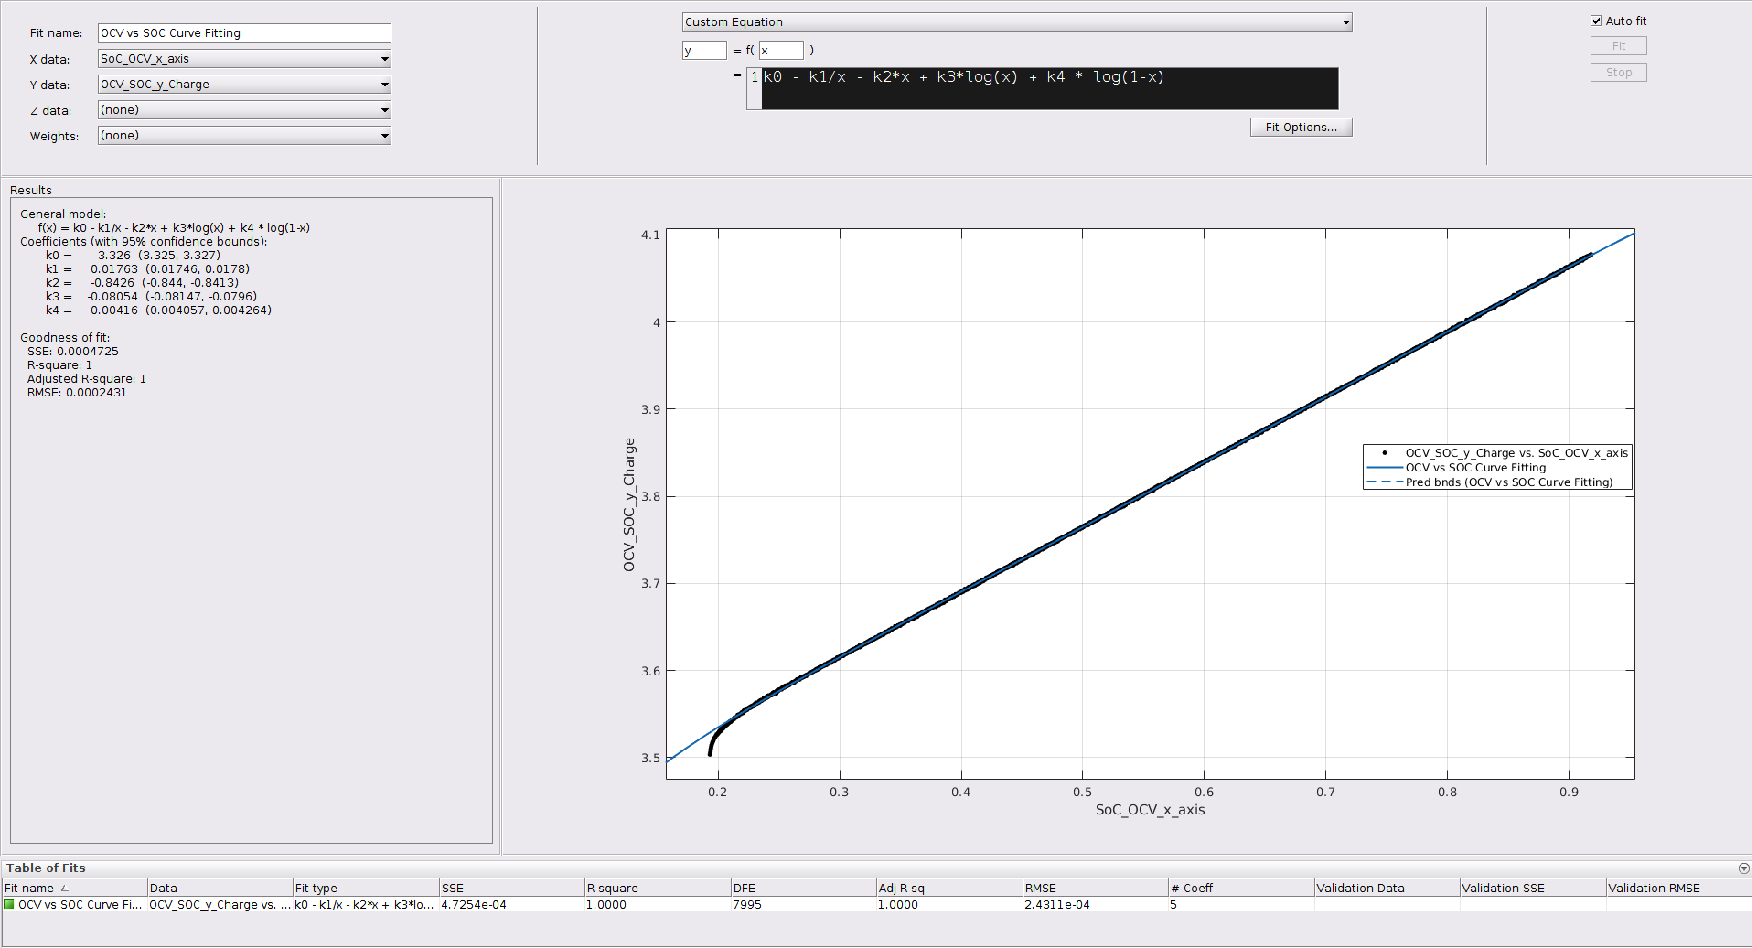
\includegraphics[width=1.0\textwidth, keepaspectratio]{images/Curve_Fitting_2.pdf}
	\caption{MATLAB Curve Fitting Toolbox for Model - 2}
	\label{fig:OCV_SOC_Model_2}
\end{figure}

\begin{table}[h]
	\center
	\begin{tabular}{||c | c | c | c ||} 
		\hline
		Coefficient & Value with 95\% Confidence Bounds & Lower Bound & Upper Bound \\ [0.5ex] 
		\hline\hline
		$K_{0}$ & $3.326$  & $-\infty$ & $\infty$ \\ 
		\hline
		$K_{1}$ & $0.01763$ & $-\infty$ & $\infty$ \\
		\hline
		$K_{2}$ & $-0.8426$ & $-\infty$ & $\infty$ \\
		\hline
		$K_{3}$ & $-0.08054$ & $-\infty$ & $\infty$ \\
		\hline
		$K_{4}$ & $0.00416$ & $-\infty$ & $\infty$ \\
		\hline
	\end{tabular}
	\caption{\label{table:OCV_SOC_Model_2_1}Coefficients of the model-2 with bounds.}
\end{table}

\begin{table}[h]
	\center
	\begin{tabular}{||c | c | c | c ||} 
		\hline
		SSE & RMSE & R-Square & Adjusted R-sq\\ [0.5ex] 
		\hline\hline
		$0.0004725$ & $0.0002431$  & $1$ & $1$ \\ 
		\hline
	\end{tabular}
	\caption{\label{table:OCV_SOC_Model_2_2}The Goodness of fit of the model-2.}
\end{table}

\subsection{Model-3} \label{Model-3}
It can be understood that the last model, Model-3  is somehow a simplified version of Model-1 \ref{Model-1}. Usage of this model can be found in a few studies \cite{Neumann2011}.  In this model number of parameters are reduced to four. OCV-SOC relation in the model is indicated at the following equation:

\begin{figure}[]
	\centering
	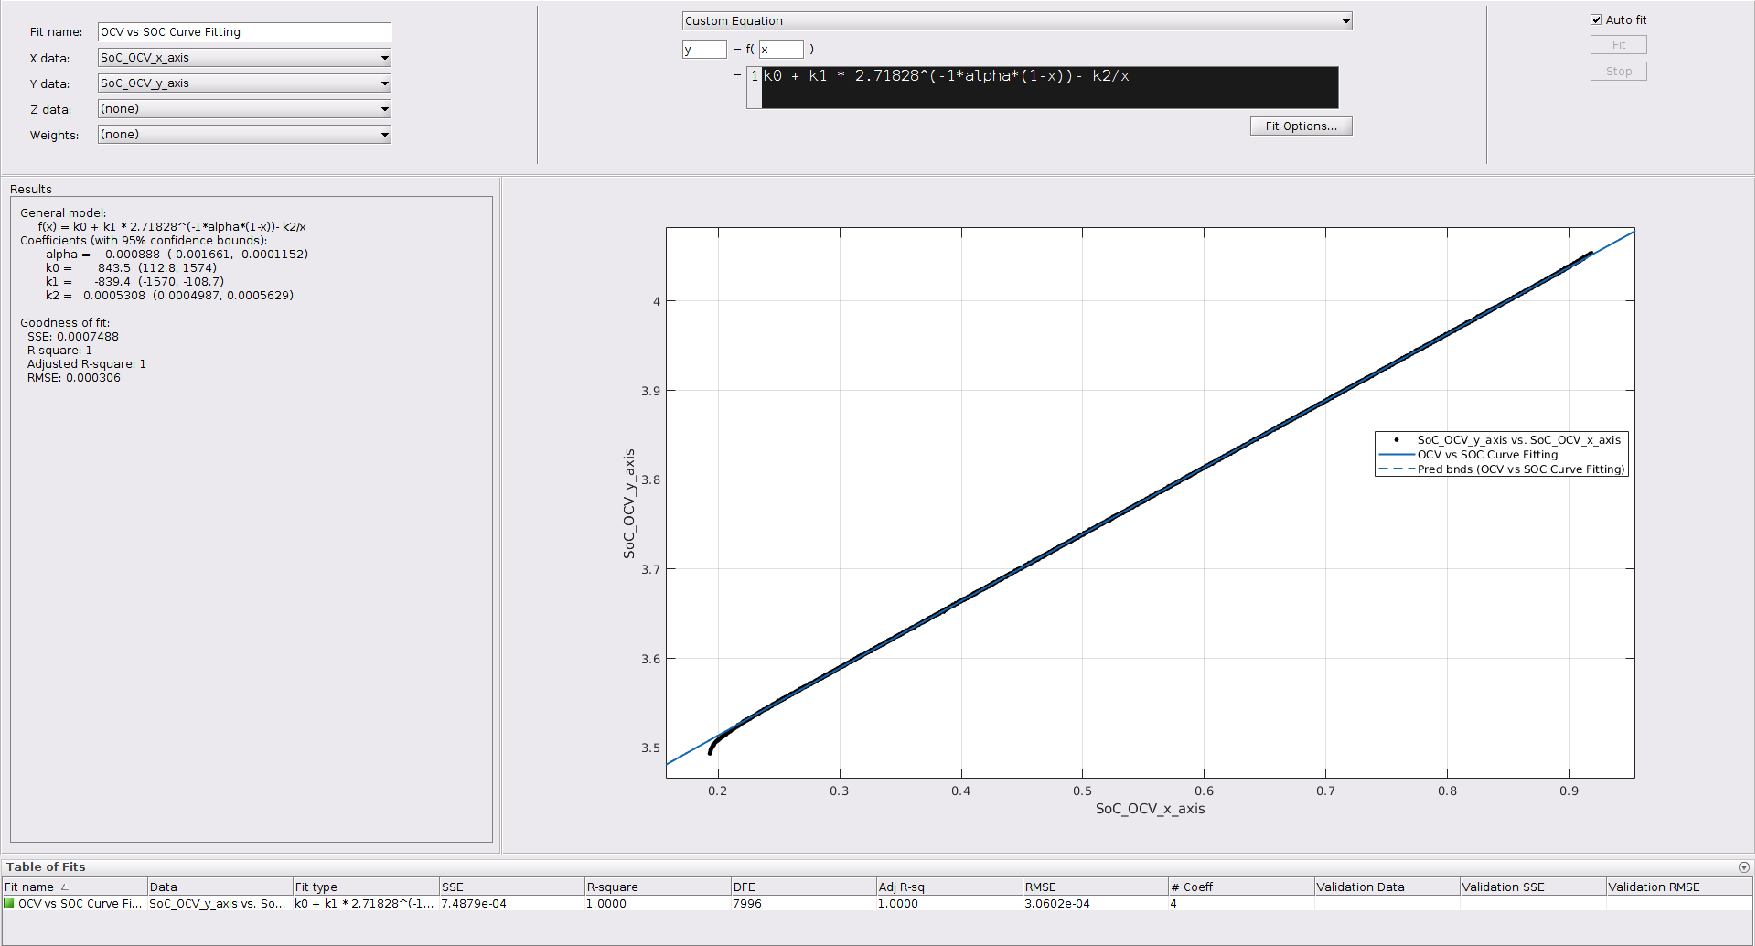
\includegraphics[width=1.0\textwidth, keepaspectratio]{images/Curve_Fitting_3.pdf}
	\caption{MATLAB Curve Fitting Toolbox for Model - 3}
	\label{fig:OCV_SOC_Model_3}
\end{figure}
\vspace{-2mm}
\begin{equation}
	\label{eqn:OCV_SOC_Model_3}
	U_{OC}(SOC(t)) = K_{0} + K_{1}{\exp}^{-\alpha(1-SOC(t))} - \frac{K_{2}}{SOC(t)}
\end{equation}

\par \noindent Parameters of the above function, \ref{eqn:OCV_SOC_Model_3},  is found via \textbf{NonlinearLeastSquare} method and \textit{Trust-Region} algorithm within the pretty large boundary. Coefficients is calculated with 95\% confidence bounds. Value of irrational number $e$, also represented as $\exp$ is taken as $2.71828$ in order to obtain an approximate solution. Table \ref{table:OCV_SOC_Model_3_1} shows the coefficient values and their limits and next Table \ref{table:OCV_SOC_Model_3_2} includes the sum of the squared prediction errors (SSE), the root mean square error (RMSE), R-square (i.e. it is a statistical measure of how close the data are to the fitted regression line), and adjusted R-sq.
\vspace{-2mm}
\begin{table}[!h]
	\center
	\begin{tabular}{||c | c | c | c ||} 
		\hline
		Coefficient & Value with 95\% Confidence Bounds & Lower Bound & Upper Bound \\ [0.5ex] 
		\hline\hline
		$\alpha$ & $-0.000888$  & $-\infty$ & $\infty$ \\ 
		\hline
		$K_{0}$ & $843.5$ & $-\infty$ & $\infty$ \\
		\hline
		$K_{1}$ & $-839.4$ & $-\infty$ & $\infty$ \\
		\hline
		$K_{2}$ & $0.0005308$ & $-\infty$ & $\infty$ \\
		\hline
	\end{tabular}
	\caption{\label{table:OCV_SOC_Model_3_1}Coefficients of the model-3 with bounds.}
\end{table}

\begin{table}[!h]
	\center
	\begin{tabular}{||c | c | c | c ||} 
		\hline
		SSE & RMSE & R-Square & Adjusted R-sq\\ [0.5ex] 
		\hline\hline
		$0.0007488$ & $0.000306$  & $1$ & $1$ \\ 
		\hline
	\end{tabular}
	\caption{\label{table:OCV_SOC_Model_3_2}The Goodness of fit of the model-3.}
\end{table}

\section{Determination of Nominal Capacity, $Q$}
\label{Total_Capacity_Calculation}
\lstinputlisting{MATLAB_Files/Total_Capacity_Explanation.m} 

\section{The Relation Between RLS Parameters and Equivalent Circuit Parameters} \label{Relation_RLS_Parameter_Circuit_Parameter} 
Equation \ref{eqn:transfer_function_Laplace_domain} is rewritten in explicit form as follows: %\cite{Xiangdong2019}:

\begin{equation}
	\label{eqn:transfer_function_Laplace_domain_2}
	G(s) = -\dfrac{R_{0}s^{2} + \dfrac{R_{0}R_{1}C_{1}+R_{0}R_{2}C_{2}+R_{2}R_{1}C_{1}+R_{1}R_{2}C_{2}}{R_{1}C_{1}R_{2}C_{2}}s+\dfrac{R_{0}+R_{1}+R_{2}}{R_{1}C_{1}R_{2}C_{2}}}{s^2 + \dfrac{R_{1}C_{1}+R_{2}C_{2}}{R_{1}C_{1}R_{2}C_{2}}s + \dfrac{1}{R_{1}C_{1}R_{2}C_{2}}}
\end{equation}

\noindent Using the bilinear transformation equation that is already given at \ref{eqn:bilinear_transformation}, parameters of the \ref{eqn:transfer_function_z_domain} can be formulated as:

\begin{align}
	\label{eqn:RLS_Parameters_with_RC}
	\begin{split}
		\theta_{1} =& \frac{2T^{2} - 8R_{1}C_{1}R_{2}C_{2}}{-T^{2}-2T(R_{1}C_{1}+R_{2}C_{2})-4R_{1}C_{1}R_{2}C_{2}}\\
		\theta_{2} =& \frac{T^{2}-2T(R_{1}C_{1}+R_{2}C_{2})+4R_{1}C_{1}R_{2}C_{2}}{-T^{2}-2T(R_{1}C_{1}+R_{2}C_{2})-4R_{1}C_{1}R_{2}C_{2}} \\
		\theta_{3} =& \frac{T^{2}(R_{0}+R_{1}+R_{2})+2T(R_{0}R_{1}C_{1}+R_{0}R_{2}C_{2}+R_{1}R_{2}C_{2}+R_{2}R_{1}C_{1}) + 4R_{0}R_{1}C_{1}R_{2}C_{2}}{-T^{2}-2T(R_{1}C_{1}+R_{2}C_{2})-4R_{1}C_{1}R_{2}C_{2}}\\
		\theta_{4} =& \frac{2T^{2}(R_{0}+R_{1}+R_{2})-8R_{0}R_{1}C_{1}R_{2}C_{2}}{-T^{2}-2T(R_{1}C_{1}+R_{2}C_{2})-4R_{1}C_{1}R_{2}C_{2}} \\
		\theta_{5} =& \frac{T^{2}(R_{0}+R_{1}+R_{2})-2T(R_{0}R_{1}C_{1}+R_{0}R_{2}C_{2}+R_{1}R_{2}C_{2}+R_{2}R_{1}C_{1})+4R_{0}R_{1}C_{1}R_{2}C_{2}}{-T^{2}-2T(R_{1}C_{1}+R_{2}C_{2})-4R_{1}C_{1}R_{2}C_{2}} \\ 
	\end{split}
\end{align}

\noindent The terms $T$  comes from the bi-linear transformation. Above equation, \ref{eqn:RLS_Parameters_with_RC}, may be simply rewritten with few terms. Suppose that $\textcolor{red}{a} = R_{0}$, $\textcolor{red}{b} = R_{1}C_{1}R_{2}{C}_{2}$, $\textcolor{red}{c} = R_{1}C_{1}+R_{2}C_{2}$, $\textcolor{red}{d}=R_{0}+R_{1}+R_{2}$, and $\textcolor{red}{f}=R_{0}R_{1}C_{1}+R_{0}R_{2}C_{2}+R_{1}R_{2}C_{2}+R_{2}R_{1}C_{1}$ are function of RC circuit elements. [\textbf{Note}:Notation $e$ is not chosen intentionally due to the fact that it is denoted for irrational Euler's number.]  \cite{Xiangdong2019} 

\begin{align}
	\label{eqn:RLS_Parameters_with_RC_2}
	\begin{split}
		\theta_{1} =& \frac{-2T^{2} + 8b}{T^{2} + 2cT + 4b}\\
		\theta_{2} =& \frac{4cT}{T^{2} + 2cT + 4b} - 1 \\
		\theta_{3} =& -\frac{dT^{2}+2fT + 4ab}{T^{2} + 2cT + 4b}\\
		\theta_{4} =& \frac{-2dT^{2}+8ab}{T^{2} + 2cT + 4b} \\
		\theta_{5} =& -\frac{dT^{2}-2fT+4ab}{T^{2} + 2cT + 4b} \\ 
	\end{split}
\end{align}

\noindent Therefore, previously defined $a$, $b$, $c$, $d$, and $f$ terms 
can be written in the form of parameters of the RLS estimation technique:

\begin{align}
	\label{eqn:RLS_Letters_with_RLS_Parameters}
	\begin{split}
		a =& \frac{\theta_{4}-\theta_{3}-\theta_{5}}{1+\theta_{1}-\theta_{2}} \\
		b =& \frac{T^{2}(1+\theta_{1}-\theta_{2})}{4(1-\theta_{1}-\theta_{2})} \\
		c =& \frac{T(1+\theta_{2})}{1-\theta_{1}-\theta_{2}} \\
		d =& \frac{-\theta_{3}-\theta_{4}-\theta_{5}}{1-\theta_{1}-\theta_{2}} \\
		f =& \frac{T(\theta_{5}-\theta_{3})}{1-\theta_{1}-\theta_{2}} \\
	\end{split}
\end{align}

\noindent Time constants of the circuit are the form of $\tau_{1}=\dfrac{c+\sqrt{c^2-4b}}{2}$ and $\tau_{2}=\dfrac{c-\sqrt{c^2-4b}}{2}$. Finally, the resistance and capacitance parameters can be formulated as:
\end{appendices}

\begin{align}
	\label{eqn:RLS_RC_Values_with_Letters}
	\begin{split}
		R_{0} =& a\\
		R_{1} =& \frac{\tau_{1}(d-a)+ac-f}{\tau_{1}-\tau_{2}}\\
		R_{2} =& d - a - R_{1}\\
		C_{1} =& \frac{\tau_{1}}{R_{1}}\\
		C_{2} =& \frac{\tau_{2}}{R_{2}} \\
	\end{split}
\end{align}

\subsection{Equivalent Circuit Values to Recursive Least Square Parameters}

\lstinputlisting{MATLAB_Files/RC_Values_to_RLS_Parameters.m} 
\label{Equivalent_circuit_value_to_RLCS_parameters}

\subsection{Recursive Least Square Parameters to Equivalent Circuit Values }\label{RLCS_parameters_to_equivalent_circuit_value}

\lstinputlisting{MATLAB_Files/RLS_Parameters_to_RC_Values.m} 

\section{MATLAB Code for State and Parameter Estimation}
\label{RLS_and_AEFK}
\lstinputlisting{MATLAB_Files/main_for_AEKF.m} 

\end{document}